% Options for packages loaded elsewhere
\PassOptionsToPackage{unicode}{hyperref}
\PassOptionsToPackage{hyphens}{url}
\PassOptionsToPackage{dvipsnames,svgnames*,x11names*}{xcolor}
%
\documentclass[
  a4paper]{article}
\usepackage{amsmath,amssymb}
\usepackage{lmodern}
\usepackage{setspace}
\usepackage{iftex}
\ifPDFTeX
  \usepackage[T1]{fontenc}
  \usepackage[utf8]{inputenc}
  \usepackage{textcomp} % provide euro and other symbols
\else % if luatex or xetex
  \usepackage{unicode-math}
  \defaultfontfeatures{Scale=MatchLowercase}
  \defaultfontfeatures[\rmfamily]{Ligatures=TeX,Scale=1}
\fi
% Use upquote if available, for straight quotes in verbatim environments
\IfFileExists{upquote.sty}{\usepackage{upquote}}{}
\IfFileExists{microtype.sty}{% use microtype if available
  \usepackage[]{microtype}
  \UseMicrotypeSet[protrusion]{basicmath} % disable protrusion for tt fonts
}{}
\makeatletter
\@ifundefined{KOMAClassName}{% if non-KOMA class
  \IfFileExists{parskip.sty}{%
    \usepackage{parskip}
  }{% else
    \setlength{\parindent}{0pt}
    \setlength{\parskip}{6pt plus 2pt minus 1pt}}
}{% if KOMA class
  \KOMAoptions{parskip=half}}
\makeatother
\usepackage{xcolor}
\IfFileExists{xurl.sty}{\usepackage{xurl}}{} % add URL line breaks if available
\IfFileExists{bookmark.sty}{\usepackage{bookmark}}{\usepackage{hyperref}}
\hypersetup{
  pdftitle={Development of an automatic tool for periodic surveillance of actuarial and demographic indicators},
  pdfauthor={Daniel Alonso, María Luz Durbán Reguera, Bernardo D'Auria},
  colorlinks=true,
  linkcolor={Maroon},
  filecolor={Maroon},
  citecolor={Blue},
  urlcolor={blue},
  pdfcreator={LaTeX via pandoc}}
\urlstyle{same} % disable monospaced font for URLs
\usepackage[margin=1in]{geometry}
\usepackage{color}
\usepackage{fancyvrb}
\newcommand{\VerbBar}{|}
\newcommand{\VERB}{\Verb[commandchars=\\\{\}]}
\DefineVerbatimEnvironment{Highlighting}{Verbatim}{commandchars=\\\{\}}
% Add ',fontsize=\small' for more characters per line
\usepackage{framed}
\definecolor{shadecolor}{RGB}{248,248,248}
\newenvironment{Shaded}{\begin{snugshade}}{\end{snugshade}}
\newcommand{\AlertTok}[1]{\textcolor[rgb]{0.94,0.16,0.16}{#1}}
\newcommand{\AnnotationTok}[1]{\textcolor[rgb]{0.56,0.35,0.01}{\textbf{\textit{#1}}}}
\newcommand{\AttributeTok}[1]{\textcolor[rgb]{0.77,0.63,0.00}{#1}}
\newcommand{\BaseNTok}[1]{\textcolor[rgb]{0.00,0.00,0.81}{#1}}
\newcommand{\BuiltInTok}[1]{#1}
\newcommand{\CharTok}[1]{\textcolor[rgb]{0.31,0.60,0.02}{#1}}
\newcommand{\CommentTok}[1]{\textcolor[rgb]{0.56,0.35,0.01}{\textit{#1}}}
\newcommand{\CommentVarTok}[1]{\textcolor[rgb]{0.56,0.35,0.01}{\textbf{\textit{#1}}}}
\newcommand{\ConstantTok}[1]{\textcolor[rgb]{0.00,0.00,0.00}{#1}}
\newcommand{\ControlFlowTok}[1]{\textcolor[rgb]{0.13,0.29,0.53}{\textbf{#1}}}
\newcommand{\DataTypeTok}[1]{\textcolor[rgb]{0.13,0.29,0.53}{#1}}
\newcommand{\DecValTok}[1]{\textcolor[rgb]{0.00,0.00,0.81}{#1}}
\newcommand{\DocumentationTok}[1]{\textcolor[rgb]{0.56,0.35,0.01}{\textbf{\textit{#1}}}}
\newcommand{\ErrorTok}[1]{\textcolor[rgb]{0.64,0.00,0.00}{\textbf{#1}}}
\newcommand{\ExtensionTok}[1]{#1}
\newcommand{\FloatTok}[1]{\textcolor[rgb]{0.00,0.00,0.81}{#1}}
\newcommand{\FunctionTok}[1]{\textcolor[rgb]{0.00,0.00,0.00}{#1}}
\newcommand{\ImportTok}[1]{#1}
\newcommand{\InformationTok}[1]{\textcolor[rgb]{0.56,0.35,0.01}{\textbf{\textit{#1}}}}
\newcommand{\KeywordTok}[1]{\textcolor[rgb]{0.13,0.29,0.53}{\textbf{#1}}}
\newcommand{\NormalTok}[1]{#1}
\newcommand{\OperatorTok}[1]{\textcolor[rgb]{0.81,0.36,0.00}{\textbf{#1}}}
\newcommand{\OtherTok}[1]{\textcolor[rgb]{0.56,0.35,0.01}{#1}}
\newcommand{\PreprocessorTok}[1]{\textcolor[rgb]{0.56,0.35,0.01}{\textit{#1}}}
\newcommand{\RegionMarkerTok}[1]{#1}
\newcommand{\SpecialCharTok}[1]{\textcolor[rgb]{0.00,0.00,0.00}{#1}}
\newcommand{\SpecialStringTok}[1]{\textcolor[rgb]{0.31,0.60,0.02}{#1}}
\newcommand{\StringTok}[1]{\textcolor[rgb]{0.31,0.60,0.02}{#1}}
\newcommand{\VariableTok}[1]{\textcolor[rgb]{0.00,0.00,0.00}{#1}}
\newcommand{\VerbatimStringTok}[1]{\textcolor[rgb]{0.31,0.60,0.02}{#1}}
\newcommand{\WarningTok}[1]{\textcolor[rgb]{0.56,0.35,0.01}{\textbf{\textit{#1}}}}
\usepackage{graphicx}
\makeatletter
\def\maxwidth{\ifdim\Gin@nat@width>\linewidth\linewidth\else\Gin@nat@width\fi}
\def\maxheight{\ifdim\Gin@nat@height>\textheight\textheight\else\Gin@nat@height\fi}
\makeatother
% Scale images if necessary, so that they will not overflow the page
% margins by default, and it is still possible to overwrite the defaults
% using explicit options in \includegraphics[width, height, ...]{}
\setkeys{Gin}{width=\maxwidth,height=\maxheight,keepaspectratio}
% Set default figure placement to htbp
\makeatletter
\def\fps@figure{htbp}
\makeatother
\setlength{\emergencystretch}{3em} % prevent overfull lines
\providecommand{\tightlist}{%
  \setlength{\itemsep}{0pt}\setlength{\parskip}{0pt}}
\setcounter{secnumdepth}{-\maxdimen} % remove section numbering
\usepackage{amsmath}
\usepackage{xcolor}
\ifLuaTeX
  \usepackage{selnolig}  % disable illegal ligatures
\fi
\newlength{\cslhangindent}
\setlength{\cslhangindent}{1.5em}
\newlength{\csllabelwidth}
\setlength{\csllabelwidth}{3em}
\newenvironment{CSLReferences}[2] % #1 hanging-ident, #2 entry spacing
 {% don't indent paragraphs
  \setlength{\parindent}{0pt}
  % turn on hanging indent if param 1 is 1
  \ifodd #1 \everypar{\setlength{\hangindent}{\cslhangindent}}\ignorespaces\fi
  % set entry spacing
  \ifnum #2 > 0
  \setlength{\parskip}{#2\baselineskip}
  \fi
 }%
 {}
\usepackage{calc}
\newcommand{\CSLBlock}[1]{#1\hfill\break}
\newcommand{\CSLLeftMargin}[1]{\parbox[t]{\csllabelwidth}{#1}}
\newcommand{\CSLRightInline}[1]{\parbox[t]{\linewidth - \csllabelwidth}{#1}\break}
\newcommand{\CSLIndent}[1]{\hspace{\cslhangindent}#1}

\title{Development of an automatic tool for periodic surveillance of
actuarial and demographic indicators}
\author{Daniel Alonso, María Luz Durbán Reguera, Bernardo D'Auria}
\date{July-August 2021}

\begin{document}
\maketitle

{
\hypersetup{linkcolor=}
\setcounter{tocdepth}{4}
\tableofcontents
}
\listoffigures
\setstretch{1.35}
\newpage

\hypertarget{summary}{%
\section{Summary}\label{summary}}

As a result of the COVID-19 pandemic and its large impact across Spain,
the monitoring of demographic measures as a direct result of deaths
related to such pandemic and future similarly deadly events has become
increasingly important. It is intended with this project to develop a
tool to easily monitor a selection of demographic measures. All related
to collective deaths of individuals as a result of relevant worldwide
events like the one mentioned previously, or perhaps other smaller scale
events which could increase mortality in a likely fashion.

The tool consists of an
\href{https://github.com/dreth/tfm_uc3m}{open-source}
\href{shiny.rstudio.com/}{Shiny-based} dashboard (developed in R) where
such measures are displayed in different visualizations across time. The
dashboard is containerized using Docker, in order to make possible to
run and use in in any operating system. The data is acquired from the
\href{https://ine.es/}{INE} and
\href{https://ec.europa.eu/eurostat/}{Eurostat} APIs. It is then treated
by several Python scripts and stored in a GitHub
\href{https://github.com/dreth/tfm_uc3m_data}{repository} where it can
be updated by anyone running the application.

\hypertarget{introduction}{%
\section{Introduction}\label{introduction}}

The COVID-19 pandemic has led to a widespread and noticeable temporary
increase in mortality, as well as to a reduction in life expectancy
throughout Spain. This arises a need to monitor these demographic
measures more closely and in real time.

This project consists in developing an application which allows for
active, real-time monitoring of mortality and life expectancy of the
population of Spain, through an
\href{https://github.com/dreth/tfm_uc3m}{open-source} shiny web-based
dashboard.

The application itself consists of the following functionality:

\begin{itemize}
\item
  Visualizing several mortality metrics:

  \begin{itemize}
  \tightlist
  \item
    Excess mortality
  \item
    Cumulative mortality rate
  \item
    Cumulative relative mortality rate
  \item
    Mortality improvement factor
  \end{itemize}
\item
  Visualizing life expectancy and constructing life tables
\item
  Visualizing a map of Spain with the previous metrics per autonomous
  community (CCAA)
\end{itemize}

All metrics are calculated weekly with data obtained from INE and
Eurostat, starting from the year 2010.

\newpage

\hypertarget{objectives}{%
\section{Objectives}\label{objectives}}

The main objectives of the project are the following:

\begin{itemize}
\item
  To provide an open-source, simple-to-use, web-based, OS-agnostic tool
  to compute and visualize common mortality-related metrics and life
  expectancy in time series plots, and static or interactive maps.

  \begin{itemize}
  \item
    A big focus of the project was to make this application as
    simple-to-use as possible, while maintaining the management of
    system requirements extremely low. The purpose of such approach is
    to allow virtually anyone that desires to monitor any of the metrics
    to do so by running a simple shell command. We want any user or
    institution with access to a computer and the internet to be able to
    monitor these metrics, or any such metrics which could be possibly
    added in the future without much hassle.
  \item
    An important prerequisite was to make the proyect open-source. This
    allows anyone to freely use and improve the project by adding extra
    components like other useful mortality-related measures. This makes
    the project fully auditable and free to use, modify and extend. The
    project is licensed using the
    \href{https://www.gnu.org/licenses/gpl-3.0.en.html}{GNU General
    Public License V3}.
  \end{itemize}
\item
  To provide the user with the ability to meaningfully customize the
  plot parameters.

  \begin{itemize}
  \tightlist
  \item
    The application itself should have several controls that allow the
    user to customize visualizations. Some of them are: what years to
    visualize, what metrics to visualize, what range of weeks to
    visualize (between 1 and 52), which CCAAs or age groups to
    aggregate, whether to make the plots interactive (using
    \emph{plotly}) or static (using \emph{ggplot2}), and so on.
    Different options will be available for different plots.
  \end{itemize}
\item
  To p3rovide the user the ability to download the plots and the data
  (with or without filtering).

  \begin{itemize}
  \tightlist
  \item
    The application shall include a download button with several options
    for all plots displayed within the application. The user can select
    the size of the plot from a list of predefined sizes, or specify the
    image resolution and the format from a list of available ones. We
    intend to make it so that any plot generated within the app can be
    downloaded.
  \end{itemize}
\item
  Allow the user to update and upload the data to the corresponding
  GitHub \href{https://github.com/dreth/tfm_uc3m_data}{repository}
  hosting the data, from within the application.

  \begin{itemize}
  \tightlist
  \item
    The data is constantly changing, and as soon as the data sources
    have new data available, the application will tell the user there is
    new data, and the user will be able to update the data with the
    click of a button. The updated data will be fetched, ran through the
    pipeline, and uploaded to the
    \href{https://github.com/dreth/tfm_uc3m_data}{data repository} for
    the project on GitHub. This ensures that the data is always updated
    and anyone is able to do so for everyone else from anywhere in the
    world.
  \end{itemize}
\item
  Have data updated in real-time from the official Spanish sources (INE)
  and Eurostat (also provided by INE).

  \begin{itemize}
  \tightlist
  \item
    Every time the app runs, it'll check if there's available data and
    display the most recent week for which there is data available, this
    way we allow anyone running the application to see if there is new
    data whenever the app is ran so they can update it if they desire to
    do so.
  \end{itemize}
\end{itemize}

\newpage

\hypertarget{motivation}{%
\section{Motivation}\label{motivation}}

As we saw during the COVID-19 pandemic, the most widely publicized
measures shown to the public in order to explain the status of the
pandemic and the country as a whole were always related to incidence of
the virus, death counts, recovery counts, amount of patients at ICU,
hospitalized patients by COVID-19 vs total hospitalized patients, etc.
However, \textbf{Death counts do not tell the whole story}, a death
count merely tells us that an amount of people died, it does not tell us
how much that amount of deaths affect the population. Also, \textbf{all
these measures are static}, therefore, we cannot see the effect they
cause on the population in the long term, which is where measures like
the \emph{cumulative relative mortality rate} or \emph{life expectancy}
come in, these show the impact of deaths and their long lasting effect
relative to the population over time.

As an example, 100 people dying over the course of a week within a
municipality of 10,000 inhabitants represents 1\% of the population;
that same amount of deaths would represent less than 0.01\% of the
population within a municipality of 1 million inhabitants. Therefore,
more robust measures to determine the impact of the deaths caused by a
pandemic are needed to really gauge the effect of the pandemic as a
whole.

The application allows monitoring some of these measures in real time.
Whenever it is desired to fetch new data (if available), the data can be
fetched with a click. The measures can be instantly computed with a
click and visualized to observe the evolution of the population at any
time, by age group, sex and by autonomous community (CCAA) of Spain.
Showcasing particular usefulness within events that cause large amounts
of deaths (like a pandemic, war, or heat wave) or that reduce the
general populations life expectancy (as the application can also
visualize the evolution of life expectancy over time).

\hypertarget{inspiration}{%
\subsection{Inspiration}\label{inspiration}}

The
\href{https://www.actuaries.org.uk/learn-and-develop/continuous-mortality-investigation/other-cmi-outputs/mortality-monitor}{Mortality
monitor reports} published on a weekly basis by the Institute and
Faculty of Actuaries of the UK was the strongest influece. The
application essentially offers the same metrics and more. The intention
is to improve this already quite good and useful report, make it
interactive and customizable, and localize it to Spain. Currently,
neither the INE (National Statistics Institute of Spain) or any other
Spanish institution offer these metrics along with the rest of the
features the app offers (visualizing maps, life expectancy, etc) on a
per-week basis.

The
\href{https://assets.publishing.service.gov.uk/government/uploads/system/uploads/attachment_data/file/1000512/Vaccine_surveillance_report_-_week_27.pdf}{COVID-19
vaccine surveillance report: Week 27}, published by the PHE (Public
Health England) also partly exemplifies a similar idea in its ``direct
impact on infection and mortality'' section.

\hypertarget{advantages-of-an-open-source-application-over-weekly-reports-in-pdf-format}{%
\subsection{Advantages of an open source application over weekly reports
in PDF
format}\label{advantages-of-an-open-source-application-over-weekly-reports-in-pdf-format}}

There are several advantages an application could potentially have over
static, weekly PDF reports like the one previously linked in the
\protect\hyperlink{inspiration}{Inspiration} section:

\begin{itemize}
\item
  The user has control over the visualizations, as there are controls to
  manipulate the parameters of the visualizations and interact with
  them.
\item
  The user can download the customized visualizations in their desired
  resolution or format.
\item
  The user can choose what measures of those available to show.
\item
  As the application is \href{https://github.com/dreth/tfm_uc3m}{open
  source}, developers could expand the application and add extra
  features and contribute directly to the project's development.
\item
  The measures will be as up-to-date as the data source is. As these
  reports take time to construct and analyze, they will take longer to
  be released, so the user can simply open the application and update
  the database whenever they desire to do so.
\end{itemize}

\hypertarget{why-is-monitoring-mortalitylife-expectancy-metrics-important}{%
\subsection{Why is monitoring mortality/life expectancy metrics
important?}\label{why-is-monitoring-mortalitylife-expectancy-metrics-important}}

As it is with any demographic measure, knowing general metrics about
population is important to many companies, institutions and individuals,
to list a few:

\begin{itemize}
\item
  The Government and the Ministry of Health, the main decisionmakers in
  terms of public health related issues. These two institutions can use
  these metrics to construct policies or regulations to protect the
  general health of the population, prioritize or purchase particular
  medication or medical utensils if needed, etc.
\item
  Insurance companies, those to which customers, companies, governments
  and other institutions transfer risk in order to protect themselves
  financially from health-related liabilities or death. Insurance
  companies directly use life tables to measure risk when providing life
  insurance to customers, and in order to remain profitable and offer a
  risk-assessed quality service to their customers these metrics
  modulate insurance premiums and aid in the process of decisionmaking
  when it comes to offering a policy to what the company could deem high
  or low risk customers.
\item
  Ordinary people. Perhaps mere curiosity or desire to be informed,
  being able to know in a timely manner whether the population is at
  risk or healthy helps people make choices regarding how to take care
  of themselves or how to take care of their loved ones.
\end{itemize}

\hypertarget{Metrics}{%
\section{Metrics computed by the application}\label{Metrics}}

The application's visualizations are especially focused on 3 specific
mortality metrics inspired by
\href{https://www.actuaries.org.uk/learn-and-develop/continuous-mortality-investigation/other-cmi-outputs/mortality-monitor}{the
regular rolling report by UK's Institute and Faculty of Actuaries}:

\begin{itemize}
\item
  \protect\hyperlink{CMR}{\textcolor{black}{Cumulative mortality rate}}
\item
  \protect\hyperlink{CRMR}{\textcolor{black}{Cumulative relative
  mortality rate}}
\item
  \protect\hyperlink{CMIF}{\textcolor{black}{Mortality improvement
  factor}}
\end{itemize}

Given the host of other possible metrics to be included, which are also
related to the ones previously mentioned, we decided to include the
following two additional metrics as a way to extend the capabilities of
the application:

\begin{itemize}
\item
  \protect\hyperlink{EM}{\textcolor{black}{Excess mortality}}
\item
  \protect\hyperlink{LE}{\textcolor{black}{Life expectancy}}
\end{itemize}

\newpage

\hypertarget{EM}{%
\subsection{Excess mortality}\label{EM}}

The term \emph{excess mortality} (\(EM\)) refers to a measurement which
corresponds to the difference between the average deaths which have
ocurred during the \(n\) years prior to the current \(t\) time.
Typically, the window of years to compute the average deaths is often
\(n = 5\). For the application, a window of \(n = 5\) years is used to
compute the measurement.

If excess mortality is very high and above zero, then there have been
more deaths than the previous \(n\) year average, if the number is
smaller than zero, then there have been less deaths than the previous
\(n\) year average.

Excess mortality is used to assess how many more or less deaths than the
previous years' average have ocurred. This way it's possible to
determine if there is an increase in deaths that exceed what has been
considered ``normal.''

During the COVID-19 pandemic the measurement was particularly useful as
mortality spiked beyond the expectations of pretty much any country
where the pandemic became widespread. Spain is no exception, and during
the time where the deaths were at their peak, the excess mortality of
that period of time was a highly publicized measure to illustrate how
many deaths above what usually occurs happened.

As a result of the COVID-19 pandemic, future measures calculated after
2020 must exclude 2020 and 2021 from the calculation as the death counts
are anomalous compared to previous and subsequent years prior the
COVID-19 pandemic.

For the years between 2021 and 2027 inclusive, the application uses the
same 5-year moving average used for 2020, meaning the average deaths
corresponding to week \(w\) for \(2015 \leq y \leq 2019\). After 2027 or
prior to 2021 the average death counts used are computed from the 5 year
window prior to the year(s) selected. For example, the average deaths
for \(w = 1\), 2019 will correspond to the average deaths during
\(w = 1\) for the years \(2014 \leq y \leq 2018\), and the average
deaths for \(w = 1\), 2022 will correspond to the same average deaths
observed on \(w = 1\) for the years \(2015 \leq y \leq 2019\).

The \(EM\) for week \(w\) of year \(y\) is computed as follows:

\[EM_{w, y} = \frac{D_{w, y}}{\overline{D_{w, y-5, y}}}\]

Where:

\begin{itemize}
\item
  \(D_{w, y}\): death count for week \(w\) of year \(y\)
\item
  \(\overline{D_{w, y-5, y-1}}\): average death count for week \(w\) of
  years \(y-5\), \(y-4\), \(\dots\), \(y-1\).
\end{itemize}

Exact definition:

\[EM_{w, y} = \frac{D_{w, y}}{\frac{1}{n} \sum^{n}_{k=1} D_{w, y-k}}\]

Where:

\begin{itemize}
\item
  \(D_{w, y}\): death count for week \(w\) of year \(y\)
\item
  \(n\): years to look back to, default is \(n = 5\)
\item
  \(D_{w, y-k}\): death count for week \(w\) of year \(y-k\), where
  \(k\) starts at \(k=1\) and ends at \(n\) with \(k \in \mathbb{N}\).
\end{itemize}

We can see an example of the most generalized \(EM\) plot the
application can produce:

\begin{figure}
\centering
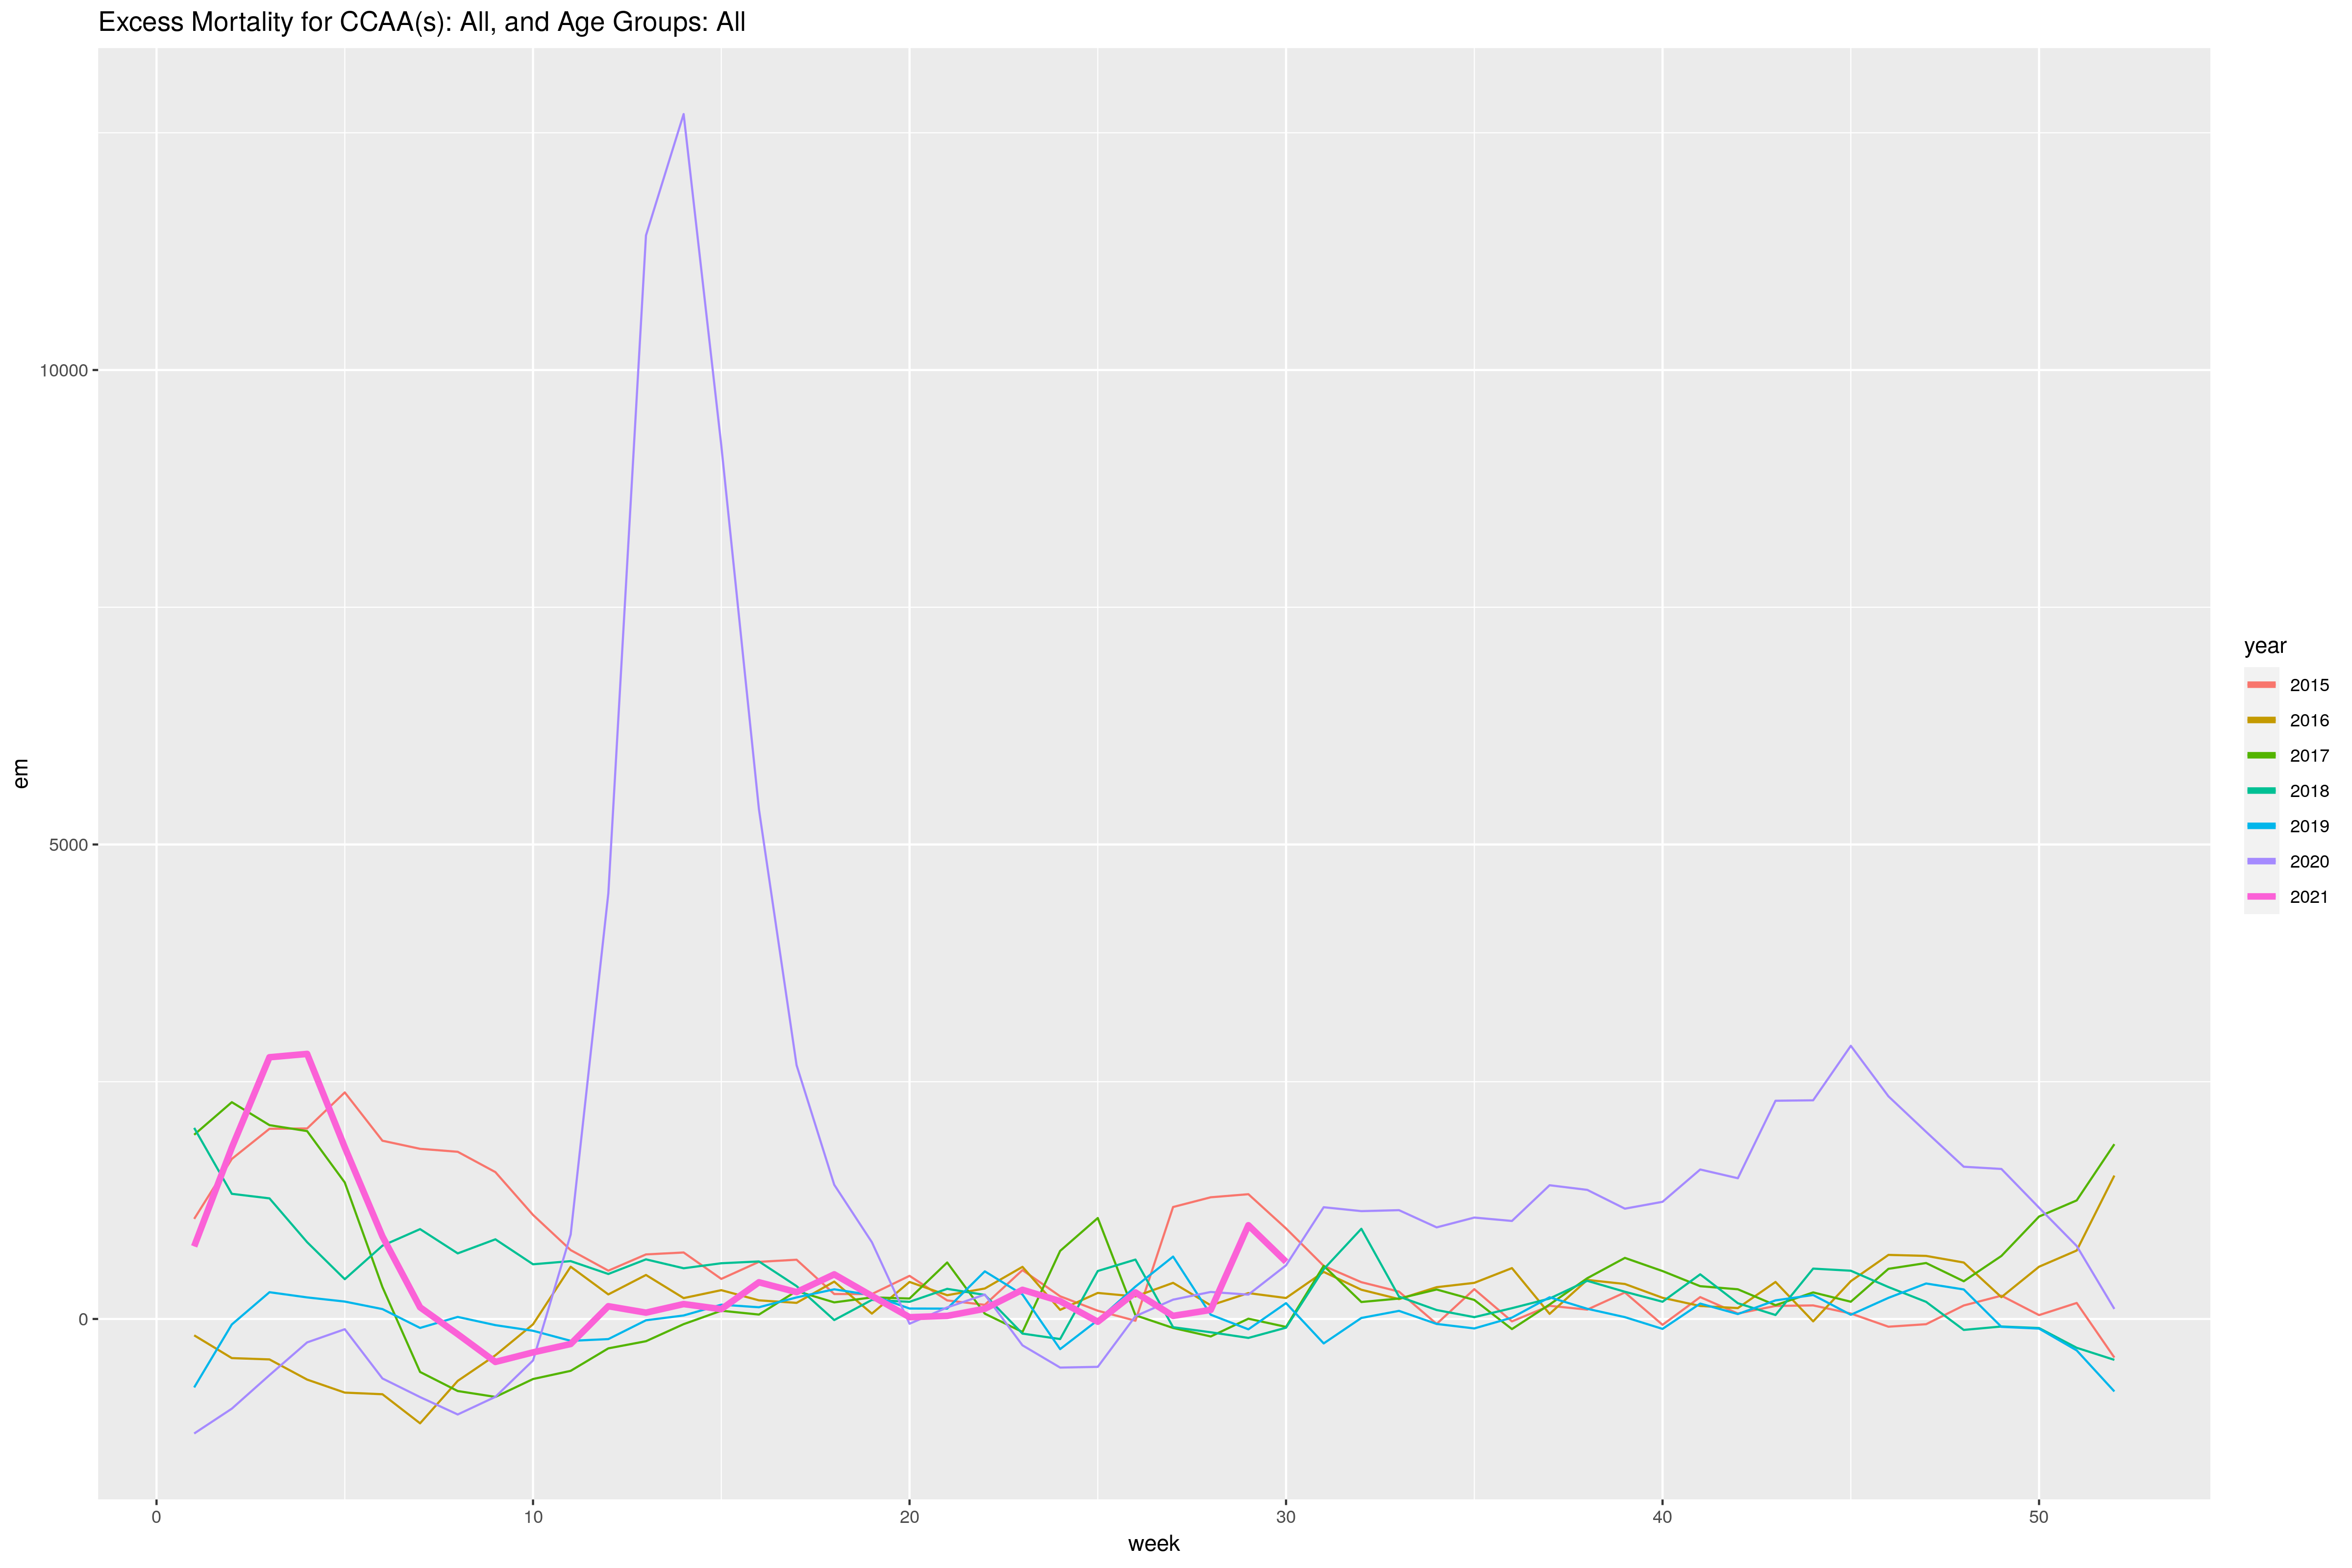
\includegraphics{./images/em.png}
\caption{Excess mortality, from 2015 up to week 30 of 2021}
\end{figure}

In Figure 1, we can clearly notice a pattern where 2020 severely
exceeded the mortality expected value of the previous 5 years.
Particularly during the 1st wave of COVID-19 (around march, april and
may), and towards the end of the year (around october, november and
december).

\newpage

\hypertarget{CMR}{%
\subsection{Cumulative mortality rate}\label{CMR}}

The \emph{cumulative mortality rate} (\(CMR\)) represents the ratio
between the sum of all deaths during the first week of a year up to a
user-defined week of the same year, and the population at that same
user-defined week and year, where weeks must be \(1 \leq w \leq 52\).

This ratio can be used standalone to gauge the amount of deaths in a
time period divided by the population alive at that time period, but, it
is most commonly used in this project as a component of the more
informational
\emph{\protect\hyperlink{CRMR}{\textcolor{black}{cumulative relative
mortality rate}}} or
\emph{\protect\hyperlink{CMIF}{\textcolor{black}{mortality improvement
factor}}}.

The ratio is computed, depending on user selection, for years stretching
as far back as 2010 and as updated as the current year. It can only be
computed for any specified range between 1 and week \(w\).

The \(CMR\) for year \(y\) and up to week \(s\) is computed as follows:

\[CMR_{w, y} = \frac{\sum^{s}_{w=1} D_{w, y}}{P_{w, y}}\]

Where:

\begin{itemize}
\item
  \(D_{w, y}\): death count for week \(w\) of year \(y\).
\item
  \(P_{w, y}\): population at week \(w\) of year \(y\)
\item
  \(s\): upper bound of week for which the death count is computed, with
  \(1 \leq s \leq 52\) and \(s \in \mathbb{N}\).
\end{itemize}

Here we see an example of the \(CMR\) time series computed by the
application:

\begin{figure}
\centering
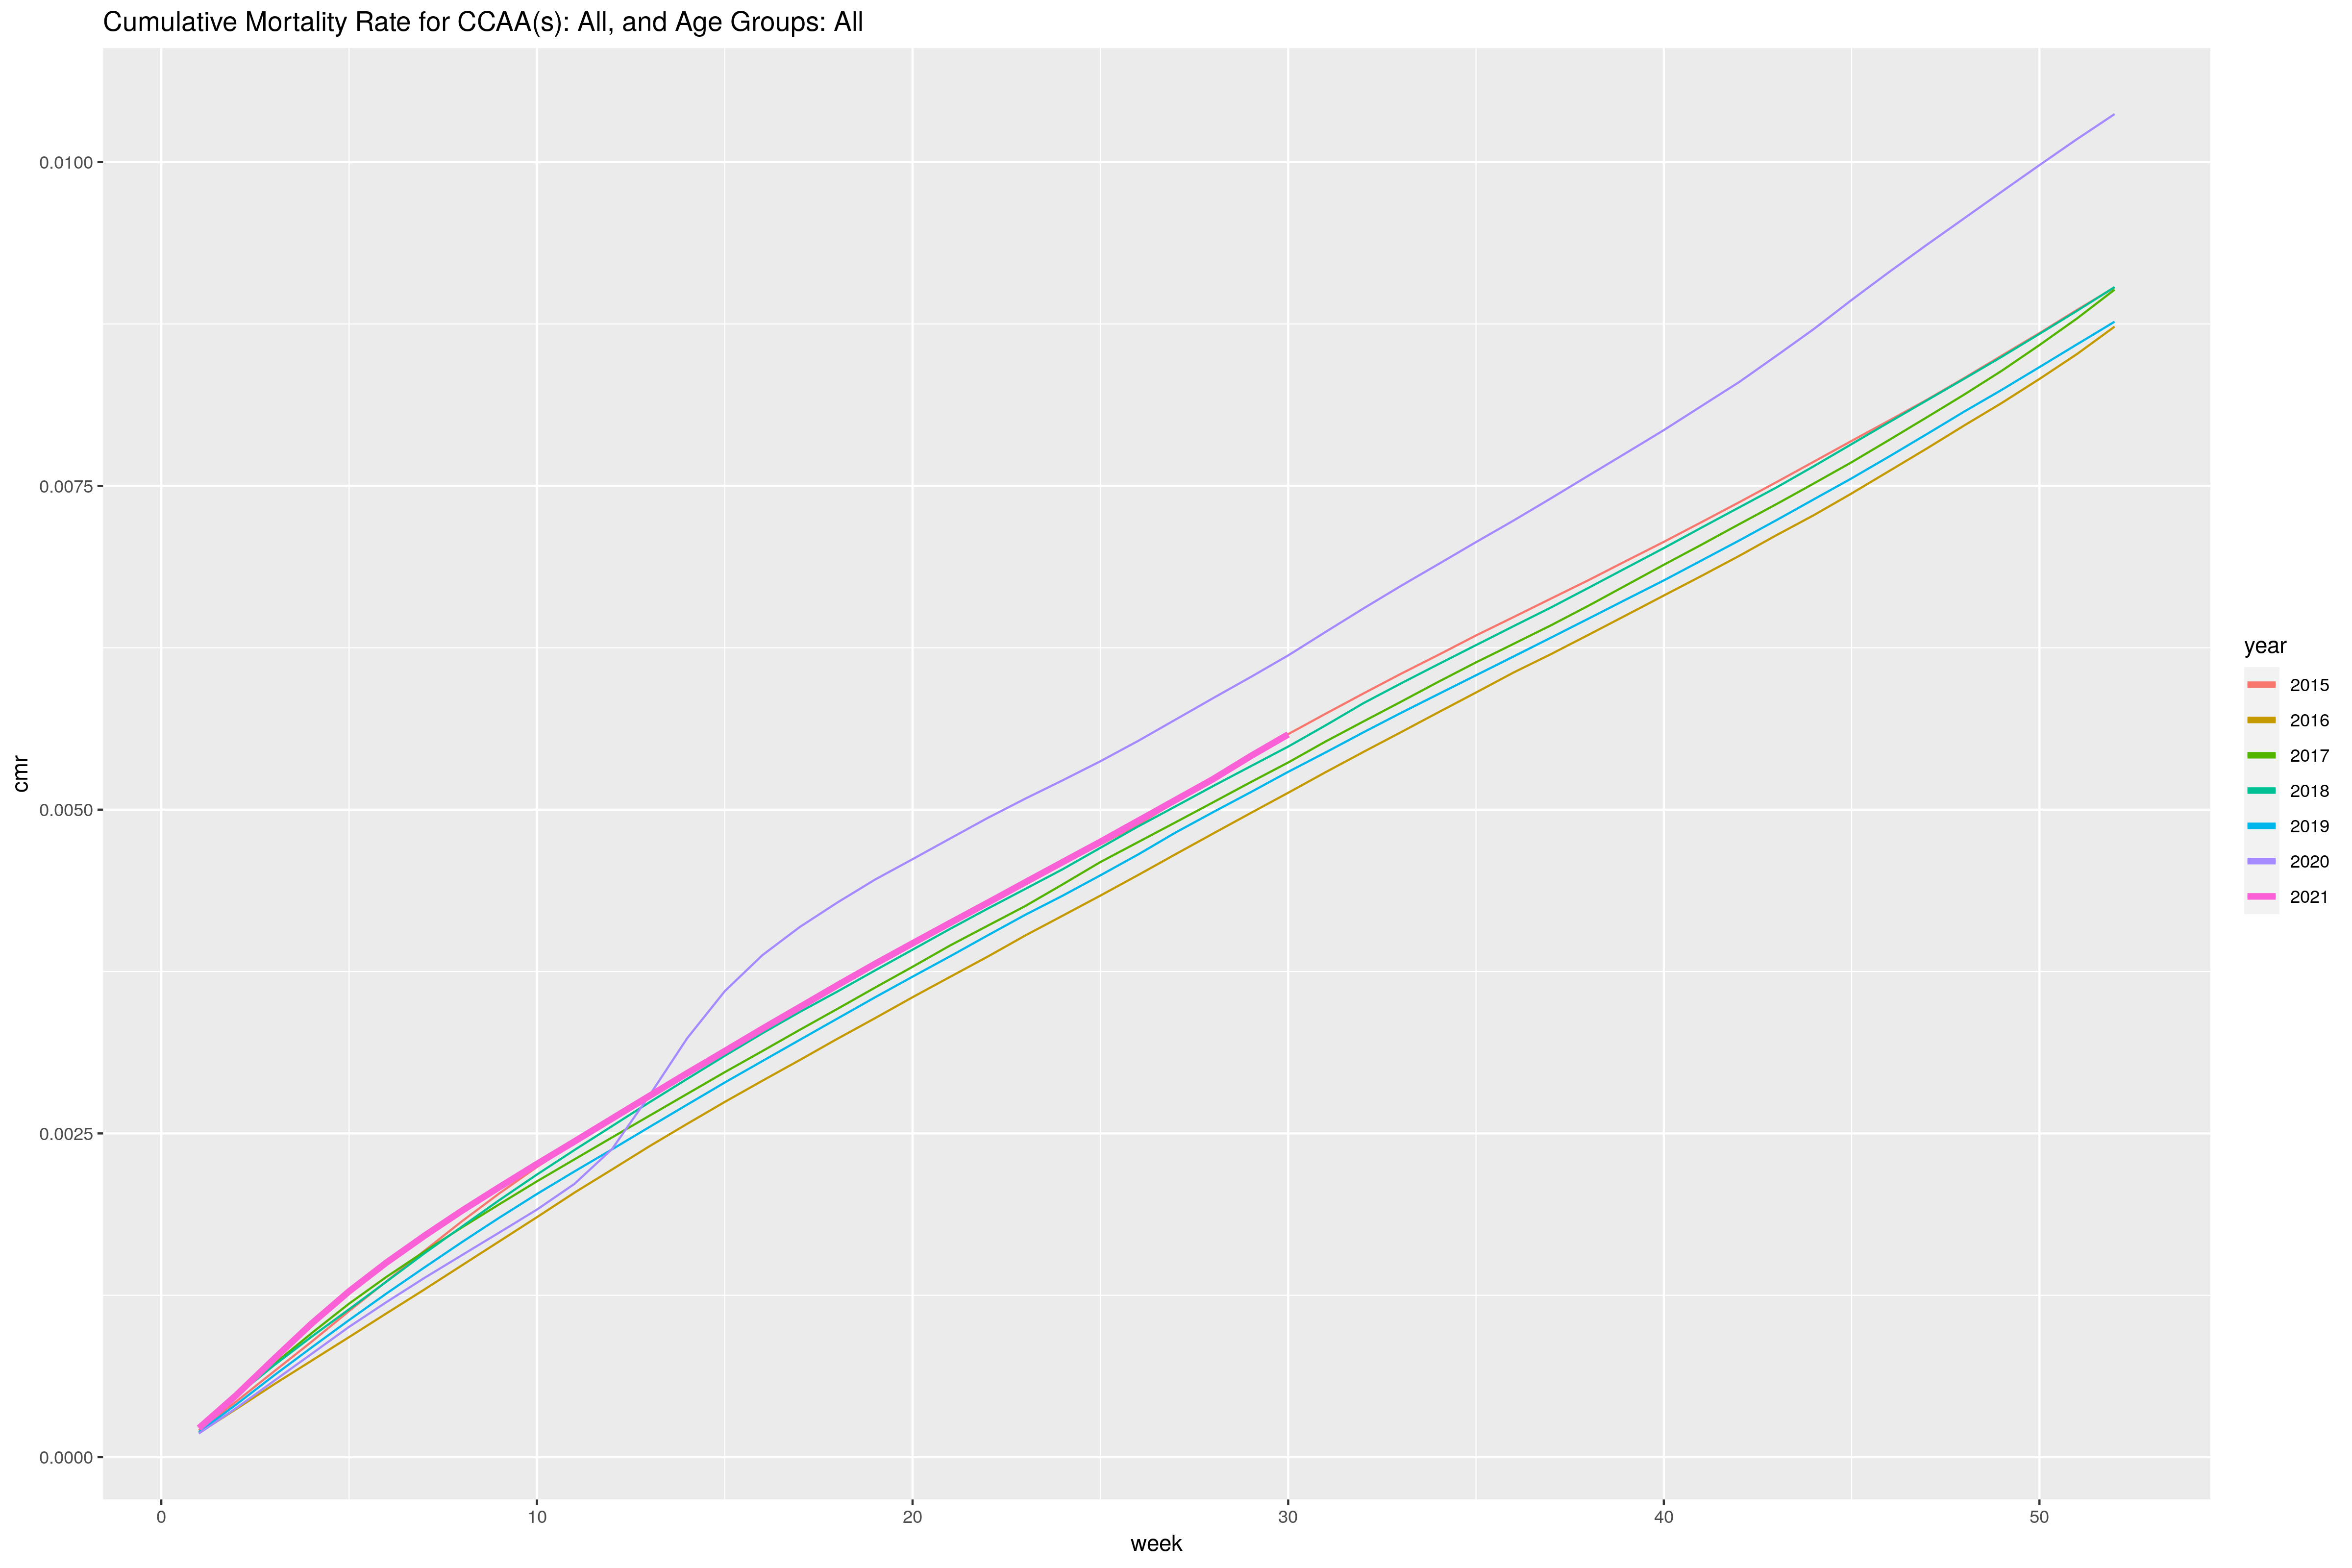
\includegraphics{./images/cmr.png}
\caption{\(CMR\), from 2015 up to week 30 of 2021}
\end{figure}

Figure 2, in contrast to the Figure 1 shows the long term cumulative
effect of increased mortality. Here 2020 rises above every other year in
terms of \(CMR\). We can also see 2021 showing a meaningful recovery
from 2020 but following the path of 2015, which prior to the arrival of
the pandemic was considered a particularly bad year in terms of
mortality.

\hypertarget{CRMR}{%
\subsection{Cumulative relative mortality rate}\label{CRMR}}

The \emph{cumulative relative mortality rate} (\(CRMR\)) corresponds to
the ratio of the difference between the cumulative mortality rate
(\(CMR\)) at a specified week and the average \(CMR\) between years
\(n-k\) and \(n-1\) inclusive, and the average \(CMR\) in that same
range of years for their last week (the 52nd week).

The \(CRMR\) allows us to show the medium to long-term effect of
catastrophic or mortality-rising events on the population based on the
\(CMR\).

The effect of long-lasting events like the COVID-19 pandemic clearly
show how mortality can part away from the mean significantly and how the
cumulative effect of such mortality can rise to unprecedented levels for
relatively long periods of time.

This particular metric can be affected significantly by events which we
might perceive as not-so-dramatic when they occur (perhaps like a severe
heat wave), but it lets us historically see how much worse or better (in
terms of mortality) a given time period can be.

In our particular case, the metric has been computed using the average
\(CMR\) for years between 2010 and 2019. 2020 is explicitly excluded, as
the effect of the COVID-19 pandemic would skew our perspective on 2021
mortality and further years.

The \(CMR\) for the last week of those years is averaged as it includes
the entire year, given that the CMR is computed for a range of weeks
starting at week 1 and ending at week \(s\), for this metric we compute
the denominator for week \(s=52\) and the numerator for a specified week
range.

The \(CRMR\) for week \(w\) of year \(y\) has been computed as follows:

\[CRMR_{w, y} = \frac{CMR_{w, y} - \frac{1}{10} \sum^{2019}_{y=2010} CMR_{w, y}}{\frac{1}{10} \sum^{2019}_{y=2010} CMR_{w=52, y}}\]

Where:

\begin{itemize}
\tightlist
\item
  \(CMR_{w, y}\) is the \emph{cumulative mortality rate} at week \(w\)
  of year \(y\)
\end{itemize}

Here is an example plot of the \(CRMR\) we can generate for all age
groups, sexes and CCAA aggregated:

\begin{figure}
\centering
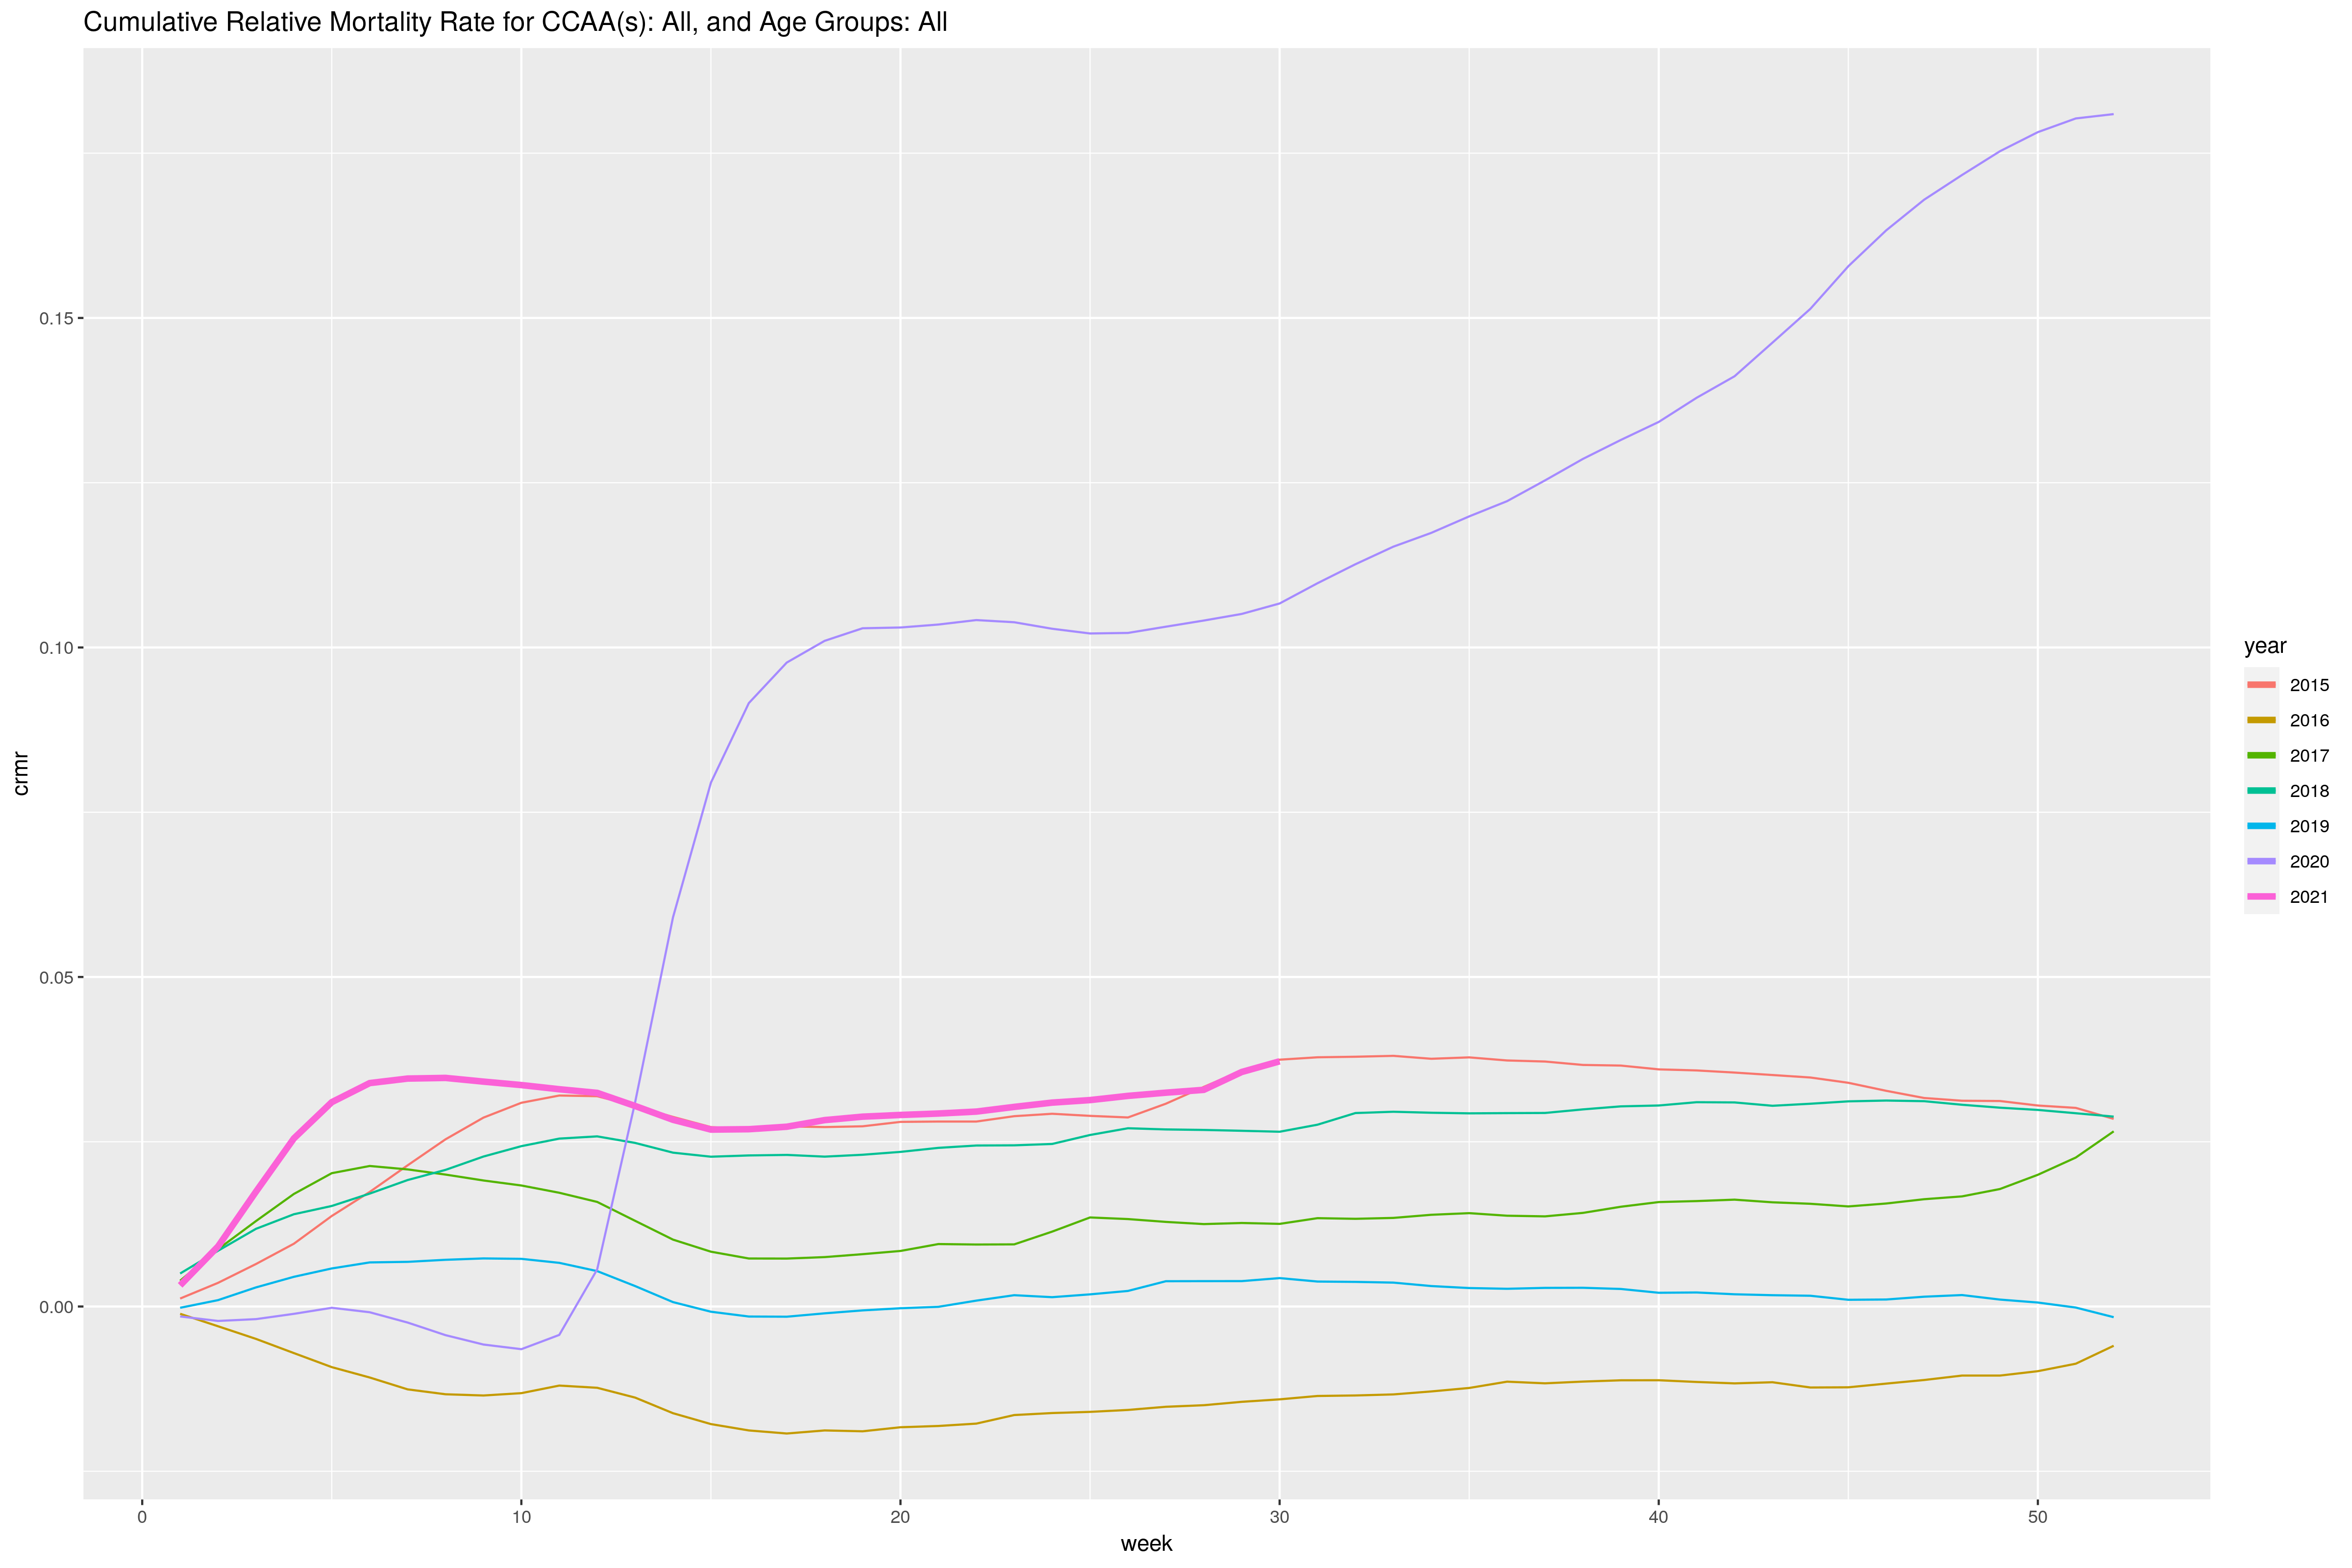
\includegraphics{./images/crmr.png}
\caption{\(CRMR\), from 2015 up to week 30 of 2021}
\end{figure}

As we can notice in Figure 3, 2020 severely exceeded the previous years'
\(CRMR\) throughout the year right after the pandemic started, and the
trend was sustained throughout the whole year. The dramatic increase
towards the first wave of the pandemic completely skews the y-axis scale
of the plot. We can also notice how the start of 2021 was also out of
the ordinary, eventually returning to levels seen around 2015 (a year
previously considered particularly bad for mortality in Spain), as the
pandemic has continued to extend, but with a significantly smaller
\(CRMR\) than that of 2020 given the widespread vaccinations and more
experienced treatment of the virus.

\newpage

\hypertarget{CMIF}{%
\subsection{Cumulative mortality improvement factor}\label{CMIF}}

The \emph{cumulative mortality improvement factor} (\(CMIF\)) at a
specific week \(w\) of a year \(y\) is an actuarial measure defined as
the ratio of the difference between the \(CMR\) at week \(w\) for the
previous year \(y-1\) and the \(CMR\) at week \(w\) for the current year
\(y\), and the \(CMR\) at week 52 for the previous year \(y-1\).

The \(CMIF\) is used to assess how much mortality is improving within
specific age ranges, or the population as a whole. By ``improvement
factor'' we mean that it could either get ``better'' or get ``worse,''
the ``better'' the \(CMIF\) gets, the lower the mortality is, the
``worse'' it gets, the opposite, meaning mortality will be higher.

This measure is an excellent one when it comes to determining a
population's longevity. If the improvement factor is high, then the
older the population can become, in some ways, very similarly to life
expectancy.

The metric is particularly useful for older age groups, which during the
COVID-19 pandemic saw a significant increase in mortality as a result of
it being a virus especially dangerous to older age groups and it also
being very easily spread throughout populations. In Spain in particular,
retirement homes are very commonly used to house retired elderly people.
The virus was unfortunately spread among some retirement homes causing
very high mortality. These events directly affect the improvement factor
negatively. Improvement factors are especially useful in insurance,
where they're often used to compute projections for life insurance
policies.

For the application in particular, the \(CMIF\) can be computed for
years above 2011, as the data only stretches as far back as 2010 and the
measure looks back 1 year.

The \(CMIF\) for week \(w\) of year \(y\) is computed as follows:

\[CMIF_{w, y} = \frac{CMR_{w, y-1} - CMR_{w, y}}{CMR_{w=52, y-1}}\]

Where:

\begin{itemize}
\tightlist
\item
  \(CMR_{w, y}\) is the \emph{cumulative mortality rate} at week \(w\)
  of year \(y\)
\end{itemize}

\newpage

As a way to exemplify, we can also show a plot for the \(CMIF\), as
plotted through the application:

\begin{figure}
\centering
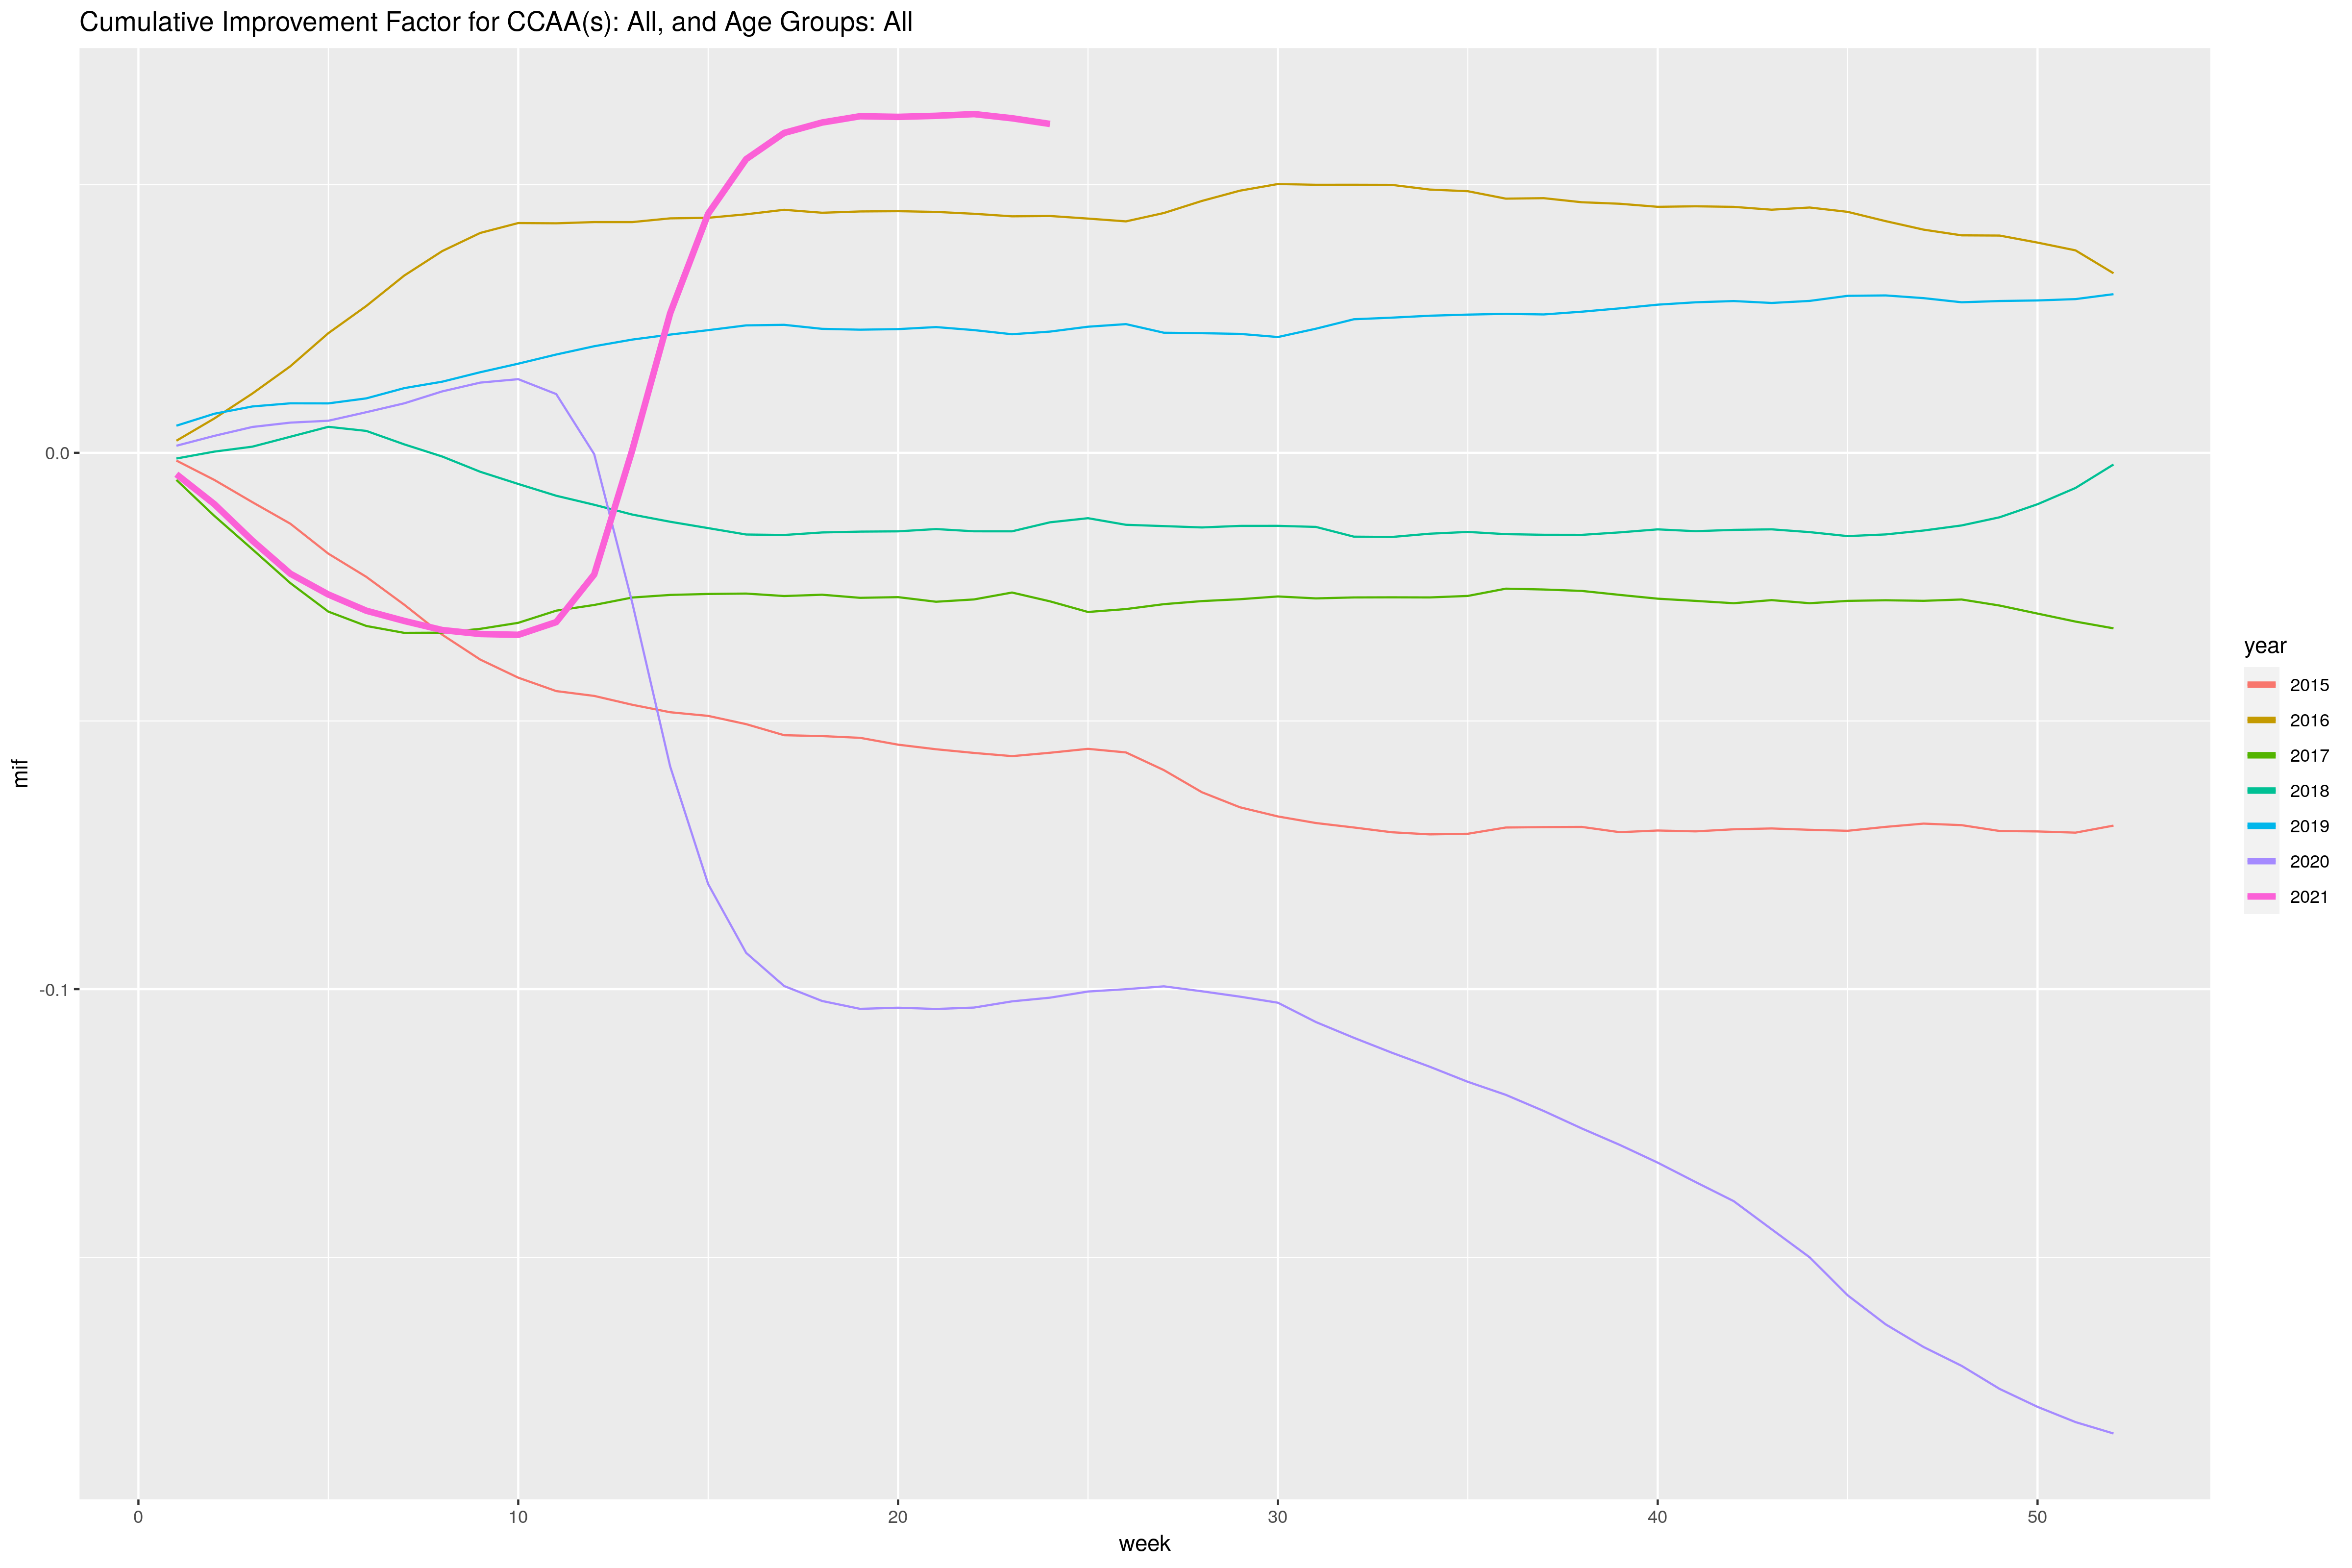
\includegraphics{./images/cmif.png}
\caption{\(CMIF\), from 2015 up to week 30 of 2021}
\end{figure}

As for the \(CMIF\) visualized in Figure 4, it is clear how significant
the decline of the \(CMIF\) is for 2020, and how noticeable of an
improvement the widespread vaccination has been during 2021.

Comparatively we can say that rises in \(CRMR\) correspond with declines
in \(CMIF\).

\hypertarget{LE}{%
\subsection{Life expectancy}\label{LE}}

\emph{Life expectancy} (\(LE\)) is a measure that estimates the time an
organism is expected to live. It is computed for a specific age group
\(A\) using a \emph{life table}, which is a table commonly used in
actuarial science, demography and life insurance policy risk modelling
that shows the probability that a person of a certain age or age group
will die before reaching their next birthday or entering the next age
group. The last column of it commonly corresponds with the \emph{life
expectancy} for that age or age group based on that probability of
death.

\(LE\) at birth would correspond to the \(LE\) of the youngest age group
in the table, assumming we don't have the \emph{infant mortality rate}
(\(IMR\)).

The purpose of this measure is to track how long we should expect our
population to live. As an upper limit on how old we should expect the
population to become. It is widely used in insurance to calculate
insurance premiums on life insurace policies, and to determine if it's
even profitable to offer such policies to an individual. A very old
individual would be surcharged for a life insurance policy or be
rejected altogether when attempting to acquire the policy given their
high risk of death and very low life expectancy.

It also gives us a perspective on perhaps how developed a country is,
given that most developed countries a have relatively high life
expectancy for their population.

For the purposes of this application, it is useful to track the effect
mortality has on how long we should expect the Spanish population to
live. In particular, mortality as a result of the COVID-19 pandemic has
affected life expectancy significantly, however, perhaps not in a
permanent way, as mortality eventually goes back to the mean, and with
it, so does life expectancy.

As we need to compute \(LE\) for specific weeks/years and display them
as a time series, we must then calculate a \emph{life table} per week.

The process is largely inspired from the following methodology explained
on the
\href{https://www.measureevaluation.org/resources/training/online-courses-and-resources/non-certificate-courses-and-mini-tutorials/multiple-decrement-life-tables/lesson-3.html}{MEASURE
evaluation website}. However, it was adapted to fit weekly measures by
taking data one year prior to the specified week. Calculations after the
step 2 described below are nearly identical to those displayed on the
previously linked article.

To compute \(LE\) we must first compute a life table as follows, note
that each step also corresponds to a column of the life table in the
same order:

\textbf{1.} Compute the age-specific death rate \({}_{n}m_{x}\):

\begin{equation}
{}_{n}m_{x} = \frac{\sum \text{ } {}_{x,x+n}D_{w,y}}{{}_{x,x+n}P_{w,y}}
\end{equation}

Where:

~~~~~~- \(\sum \text{ } {}_{x,x+n}D_{w,y}\) corresponds to the sum of
deaths between week \(w\) of the year \(y\) and week \(w\) of the year
\(y-1\) for individuals aged between \(x\) and \(x+n\).

~~~~~~- \({}_{x,x+n}P_{w,y}\) corresponds to the population at week
\(w\) of the year \(y\) for individuals aged between \(x\) and \(x+n\).

\textbf{2.} Compute the proportion of individuals alive at the start of
an age interval which are no longer alive at the end of that age
interval (they die at some point during the interval), \({}_{n}q_{x}\):

~~~~~~a. For non open-ended age groups:

\begin{equation}
\tag{2.1}
{}_{n}q_{x} = 1 - \frac{1}{e^{n * {}_{n}m_{x}}}
\end{equation}

~~~~~~b. For open-ended age groups (ex. 90+ year olds):

\begin{equation}
\tag{2.2}
{}_{n}q_{x} = 1
\end{equation}

Where:

\begin{itemize}
\item
  \(n\) is the length of the age interval. INE and Eurostat data is
  grouped in age interval lengths of \(n = 5\).
\item
  \(e\) is the exponential function.
\end{itemize}

\textbf{3.} Use the previously calculated measure \({}_{n}q_{x}\) to
compute \(l_x\):

~~~~~~a. For the first value we set \(l_0 = 100,000\)

~~~~~~b. For the subsequent values, we calculate the next values using
the previous one as a sequence:

\begin{equation}
\tag{3}
l_{x + n} = l_x * (1 - {}_{n}q_{x})
\end{equation}

Where:

~~~~~~- \(x\) corresponds to the numbering of the age group, (ex. for
\emph{less than 5 year olds} which is our first age group, we have
\(l_0\), then \(l_1\), and so on)

~~~~~~- \(x+n\) corresponds to the next age group after \(x\)

\textbf{4.} Compute the number of deaths ocurred within each age
interval \({}_{n}d_{x}\):

\begin{equation}
\tag{4}
{}_{n}d_{x} = l_x * {}_{n}q_{x}
\end{equation}

Where:

~~~~~~- The measure is calculated for individuals aged between \(x\) and
\(x+n\)

\textbf{5.} Calculate the person-years of life of all individuals in
each age interval \(x\) to \(x+n\), \({}_{n}L_{x}\):

\begin{equation}
\tag{5}
{}_{n}L_{x} = \frac{{}_{n}d_{x}}{{}_{n}m_{x}}
\end{equation}

\textbf{6.} We calculate the cumulative person-years of life after age
\(x\), \(T_x\). Therefore, for the first age group in the table, the
value of \(T_x\) will correspond to the sum of all \({}_{n}L_{x}\), the
entire 5th column. For the second age group, it'll be the sum of all
\({}_{n}L_{x}\) with the exception of the \({}_{n}L_{x}\) value of the
first age group, and so on.

So:

~~~~~~a. For age groups different to the last one:

\begin{equation}
\tag{6.1}
T_x = \sum^{19}_{k=g} {}_{n}L_{x}
\end{equation}

~~~~~~b. For the last age group:

\begin{equation}
\tag{6.2}
T_x = {}_{n}L_{x}
\end{equation}

Where:

~~~~~~- \(g\) is the number of the age group for which we want to
compute the measure, so for group 1, \(g=1\), and so on.

~~~~~~- The sum goes up to 19, as there are 19 age groups in our
computation.

\textbf{7.} We compute the \emph{life expectancy} (\(LE\)) of each age
group as follows:

\begin{equation}
\tag{7}
e_{x} = \frac{T_x}{l_x}
\end{equation}

Here we can see an example of the \(LE\) time series computed by the app
using the previously described methodology:

\begin{figure}
\centering
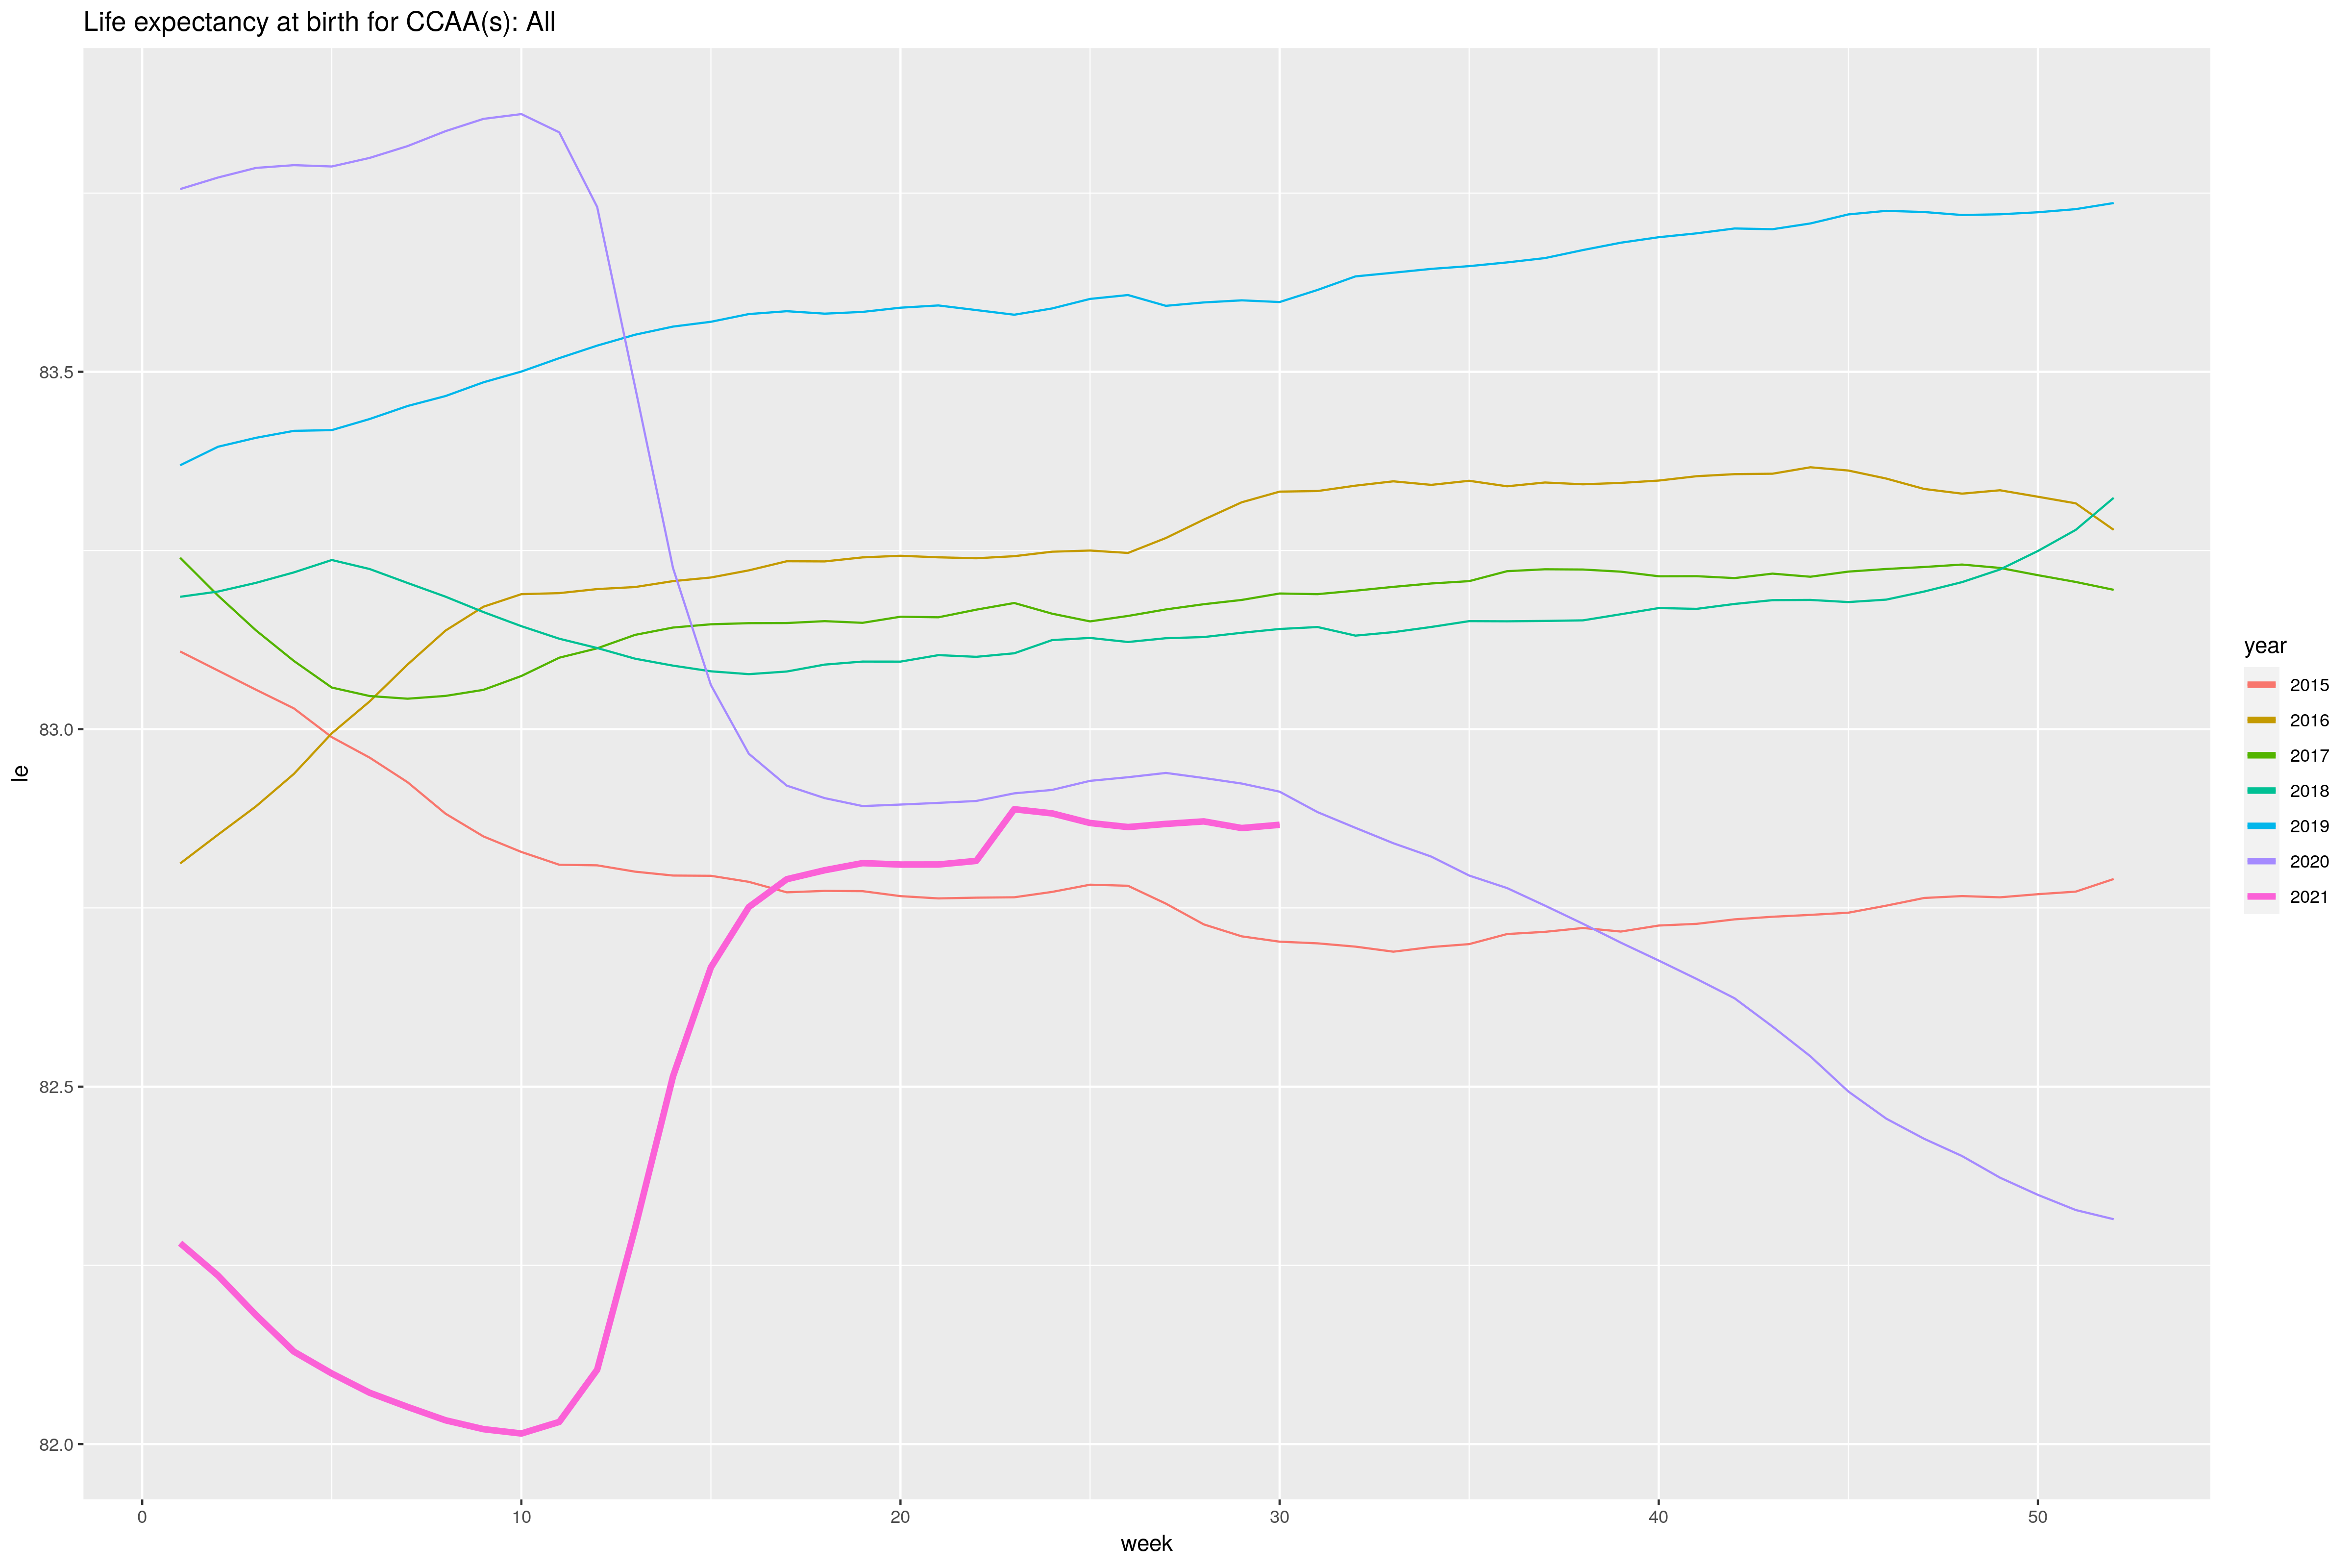
\includegraphics{./images/le.png}
\caption{Life Expectancy, from 2015 up to week 30 of 2021}
\end{figure}

We can see in Figure 5 how notably life expectancy dropped during the
pandemic, from being at its highest point in early 2020 to the lowest
point for the past 5 years. 2021 shows a recovery and return to levels
between 2015 and the period between the end of the 1st and start of the
2nd wave of COVID-19 during 2020. During the start of 2021 we also saw
the previous 5-year low recorded by late 2020 beat by an even lower low
around week 10.

\newpage

\hypertarget{technologies-used}{%
\section{Technologies used}\label{technologies-used}}

The application utilizes several tools/services to perform the entire
process of data querying, pre-processing, hosting and plotting.

\begin{itemize}
\item
  \href{https://www.python.org/}{\textbf{Python}} is an interpreted
  general-purpose object-oriented programming language. It's used within
  this project for the entirety of the data querying, pre-processing and
  updating.
\item
  \href{https://www.r-project.org/}{\textbf{R}} is a programming
  language and statistical computing environment. It's used within the
  project for the front end and back end of the dashboard, along with
  computations of all the metrics, visualizations and generation of maps
  within the application.
\item
  \href{https://www.docker.com/}{\textbf{Docker}} is a set of platform
  as a service products that use OS-level virtualization to package
  software in \emph{containers}. It's used within the project to
  containerize the application into a simple package, which allows users
  to run the application with minimal setup and by installing virtually
  no requirements (other than Docker itself). The container is also
  hosted in \href{https://hub.docker.com/r/dreth/tfm_uc3m}{Docker Hub}.
\item
  \href{https://github.com}{\textbf{GitHub}} is a hosting provider for
  software development projects and version control using Git. We use it
  to host the application's
  \href{https://github.com/dreth/tfm_uc3m}{code}, the
  \href{https://github.com/dreth/tfm_uc3m/pkgs/container/tfm_uc3m}{Docker
  container} and the \href{https://github/tfm_uc3m_data}{data} used by
  the application.
\end{itemize}

\hypertarget{data-pipelines-hosting-and-application-layout}{%
\section{Data pipelines, hosting and application
layout}\label{data-pipelines-hosting-and-application-layout}}

There are 3 key components to this application:

\begin{itemize}
\item
  \textbf{Data querying, pre-processing, hosting and updating}

  \begin{itemize}
  \tightlist
  \item
    \emph{Querying and pre-processing}: Data is obtained from the
    Eurostat and INE APIs and pre-processes using python. There's a
    pipeline for the deaths dataset (obtained from Eurostat) and a
    pipeline for the population dataset (obtained from INE).
  \item
    \emph{Hosting and updating}: After querying and pre-processing, the
    data is hosted in a data-only
    \href{https://github.com/dreth/tfm_uc3m_data}{GitHub repository},
    where it can be updated by any user of the application (as long as
    they're using the application within the Docker container).
  \end{itemize}
\item
  \textbf{Web application}: Both the front end and back end of the
  application are generated and managed using an R-based web framework
  called \href{https://shiny.rstudio.com/}{Shiny}.
\item
  \textbf{Docker container}: The application is then packaged and
  containerized in order to make it platform-agnostic using
  \href{https://docker.com}{Docker}. To view the Dockerfile that
  generates the container, see \protect\hyperlink{AppendixC}{Appendix
  C}.
\end{itemize}

\hypertarget{data-querying-and-updating}{%
\subsection{Data querying and
updating}\label{data-querying-and-updating}}

The data querying process goes over two APIs, the Eurostat API and the
INE API.

\hypertarget{eurostat-api-querying}{%
\subsubsection{Eurostat API querying}\label{eurostat-api-querying}}

In order to query the Eurostat API, we need to execute several queries
using the
\href{https://github.com/dreth/tfm_uc3m/blob/report_ref/api/functions.py\#L23}{\texttt{query\_eurostat}}
function defined in the
\href{https://github.com/dreth/tfm_uc3m/blob/main/api/functions.py}{functions.py}
script.

The queries are executed through the
\href{https://github.com/dreth/tfm_uc3m/blob/main/api/query.py\#L26}{query.py}
script upon user request.

In order to query the Eurostat API:

\begin{enumerate}
\def\labelenumi{\arabic{enumi}.}
\item
  We have to use the
  \href{https://ec.europa.eu/eurostat/web/json-and-unicode-web-services/getting-started/query-builder}{Eurostat
  Query Builder}.
\item
  Pass in the database ID, in our case it's \textbf{demo\_r\_mwk2\_05},
  we select the parameters and then query the API. The parameters can be
  concatenated.
\end{enumerate}

The previously mentioned
\href{https://github.com/dreth/tfm_uc3m/blob/report_ref/api/functions.py\#L23}{\texttt{query\_eurostat}}
function does this, thereby simplifying the process of querying by just
passing the parameters to the function as desired.

\hypertarget{death-dataset-update-pipeline}{%
\paragraph{Death dataset update
pipeline}\label{death-dataset-update-pipeline}}

As the Eurostat API returns a JSON, we must convert this response object
into a workable pandas dataframe and eventually a CSV file, for easier
storage and updating.

The pipeline followed from when the data is obtained until it's updated
the data hosted in the repository is the following, with the exception
of the \protect\hyperlink{DeathDatasetPipeline}{data manipulation
pipeline}, an intermediate step:

\begin{enumerate}
\def\labelenumi{\arabic{enumi}.}
\item
  Open the
  \href{https://github.com/dreth/tfm_uc3m/blob/main/data/logs/update_database.log}{update\_database.log}
  log file, in which diagnostic messages related to the query are
  printed temporarily until the query is over.
\item
  Create an empty list where obtained raw datasets from the API will be
  added to.
\item
  Run a nested loop where we iterate over each age group (19 age groups)
  and sex (3 sexes, male, females and total) and the Eurostat API is
  queried for each combination of sex and age group. The queried data is
  queried as far back as the data is provisional (Week 1, 2020 at the
  time of writing).
\item
  Each obtained dataset is passed through the
  \href{https://github.com/dreth/tfm_uc3m/blob/report_ref/api/functions.py\#L84}{\texttt{generate\_death\_df}}
  function defined in the
  \href{https://github.com/dreth/tfm_uc3m/blob/main/api/functions.py}{functions.py}
  script, which runs the steps described in the
  \protect\hyperlink{DeathDatasetPipeline}{pipeline for the death
  dataset} section. Thereby generating a partial dataset for the current
  \emph{age+sex} looping combination.
\item
  The previously generated partial dataset is added to the
  \href{https://github.com/dreth/tfm_uc3m/blob/main/api/query.py\#L31}{\texttt{death\_datasets}}
  list created previously.
\item
  The datasets within the
  \href{https://github.com/dreth/tfm_uc3m/blob/main/api/query.py\#L48}{\texttt{death\_datasets}}
  list are all concatenated using the
  \href{https://pandas.pydata.org/pandas-docs/stable/reference/api/pandas.concat.html}{\texttt{pandas.concat}}
  function.
\item
  The updated dataset is passed as a parameter of the
  \href{https://github.com/dreth/tfm_uc3m/blob/main/api/query.py\#L51}{\texttt{perform\_update\_datasets}}
  function defined in the
  \href{https://github.com/dreth/tfm_uc3m/blob/report_ref/api/functions.py\#L447}{functions.py}
  script, which in turn checks the currently available dataset within
  the repository file tree, imports it, updates all the provisional data
  and appends the newly obtained data if available.
\item
  The acquired/updated dataset is exported as a CSV file.
\end{enumerate}

\hypertarget{ine-api-querying}{%
\subsubsection{INE API querying}\label{ine-api-querying}}

To query the INE API, a single query is executed using the
\href{https://github.com/dreth/tfm_uc3m/blob/report_ref/api/functions.py\#L146}{\texttt{query\_INE\_pop}}
function defined in the
\href{https://github.com/dreth/tfm_uc3m/blob/main/api/functions.py}{functions.py}
script.

The function executes a single query with data starting at the date
defined by the \emph{start} parameter of the function, whose default
value is \emph{20100101}, corresponding to the 1st of January, 2010.
This single query returns a JSON response with all the data.

In order to query from INE we have to use their
\href{https://www.ine.es/dyngs/DataLab/en/manual.html?cid=1259945947373}{data
request} (in Spanish) methods. In particular, the ones described in the
``\emph{Obtención de datos Sistema Tempus3}'' section. In our case, we
must create a URL like:
\textcolor{green}{``\url{https://servicios.ine.es/wstempus/js/ES/DATOS_TABLA/\%7Bdf_id\%7D?date=\%7Bstart\%7D}:\{end\}''},
where \emph{df\_id} is the ID of the database (\textbf{9681} for us),
and \emph{start} being where the time series will start and \emph{end}
where it will end. If \emph{end} is left empty, then it'll fetch the
most recent data.

\hypertarget{population-dataset-update-pipeline}{%
\paragraph{Population dataset update
pipeline}\label{population-dataset-update-pipeline}}

The INE API returns a JSON file with somewhat unique formatting,
therefore, in order to generate a clean dataset and update the database
with the cleaned up dataset, we need to go through a few steps. The
intermediate step detailing the cleaning and pre-processing pipeline is
detailed in the \protect\hyperlink{PopDatasetPipeline}{data
pre-processing pipeline} section for the population dataset.

\begin{enumerate}
\def\labelenumi{\arabic{enumi}.}
\item
  Gather the latest week updated in the death dataset and assign it to
  the
  \href{https://github.com/dreth/tfm_uc3m/blob/main/api/query.py\#L49}{\texttt{most\_recent\_week}}
  object.
\item
  Open the
  \href{https://github.com/dreth/tfm_uc3m/blob/main/data/logs/update_database.log}{update\_database.log}
  log file, and log the start of the querying for the dataset.
\item
  Query the INE database using
  \href{https://github.com/dreth/tfm_uc3m/blob/main/api/query.py\#L60}{\texttt{query\_INE\_pop}}.
\item
  Run the data pre-processing pipeline using the function
  \href{https://github.com/dreth/tfm_uc3m/blob/main/api/query.py\#L61}{\texttt{generate\_pop\_df}}
  as defined in the
  \href{https://github.com/dreth/tfm_uc3m/blob/report_ref/api/functions.py\#L190}{functions.py}
  script. The steps for this pipeline are detailed its
  \protect\hyperlink{PopDatasetPipeline}{corresponding section}.
\item
  The updated dataset is passed as a parameter of the
  \href{https://github.com/dreth/tfm_uc3m/blob/main/api/query.py\#L63}{\texttt{perform\_update\_datasets}}
  function, which in turn checks the currently available dataset within
  the repository file tree, imports it, updates all the provisional data
  and appends the newly obtained data if available.
\item
  The acquired/updated dataset is exported as a CSV file.
\end{enumerate}

\hypertarget{PreProcessingPipeline}{%
\subsection{Data pre-processing pipeline}\label{PreProcessingPipeline}}

After the data is acquired, then a pipeline to convert the raw JSON
response from the APIs must be ran in order to construct actionable
dataframes to store and use for the app. In these two sections there
will be a description of all the steps in the pipeline for each of the
two datasets.

\hypertarget{DeathDatasetPipeline}{%
\subsubsection{Pipeline for the deaths
dataset}\label{DeathDatasetPipeline}}

The biggest challenge that the \emph{deaths} dataset imposed was dealing
with the indexing for the JSON response, as it had additional, and
admittedly useless or empty data entries within the JSON. Also, the data
obtained included a 53rd week for those years that don't fit the same
exact number of weeks, this must be dealt with as well.

The function that performs all these tasks is the
\href{https://github.com/dreth/tfm_uc3m/blob/report_ref/api/functions.py\#L84}{\texttt{generate\_death\_df}}
function defined in the
\href{https://github.com/dreth/tfm_uc3m/blob/main/api/functions.py}{functions.py}
script.

The pipeline steps are the following:

\begin{enumerate}
\def\labelenumi{\arabic{enumi}.}
\item
  We define a
  \href{https://github.com/dreth/tfm_uc3m/blob/report_ref/api/functions.py\#L88}{\texttt{fields}}
  dictionary to obtain all the relevant elements we want from the
  response JSON object. Each one of them corresponds to either the
  \texttt{keys} or \texttt{values} of the object, as JSONs are
  interpreted as \emph{dictionaries} in python, which makes them easier
  to work with.

  \begin{itemize}
  \tightlist
  \item
    Here we exclude weeks marked as \emph{W99} by Eurostat, which are
    basically empty values.
  \end{itemize}
\item
  The amount of values in the raw data is obtained from the length of
  the \texttt{values} key in the \texttt{fields} dictionary. The amount
  of ``region codes'' is obtained from the length of the
  \texttt{region\_codes} key in the \texttt{fields} dictionary, which
  are the CCAAs (autonomous communities of Spain). These two values are
  used to compute the amount of \emph{weeks} obtained from the raw data,
  the result of this ratio is allocated in the \texttt{weeks\_queried}
  object.
\item
  The \texttt{timeframes} key of the \texttt{fields} object that keeps
  track of the week label for each data point is cut up to the present
  date, as the current week always includes empty data. This cutoff is a
  way to keep the dataset with the same amount of data points and make
  it a multiple of the amount of CCAAs queried.
\item
  A
  \href{https://github.com/dreth/tfm_uc3m/blob/report_ref/api/functions.py\#L107}{\texttt{df}}
  dictionary is defined with its keys being the names of the columns of
  the final dataset to be outputted and its values being the values
  which the dataframe will contain with the exception of the
  \emph{year\_week} key which will later on be split into \emph{week}
  and \emph{year} columns.

  \begin{itemize}
  \tightlist
  \item
    The \emph{year\_week} column contains the values for the weeks times
    the amount of CCAAs queried, in our case, there will be 19 CCAAs
    queried, given that Spain has 19 CCAAs at the time of writing.
  \end{itemize}
\item
  The \texttt{df} dictionary is then converted into a pandas DataFrame
  and the \emph{year} and \emph{week} columns are generated from
  splitting the \emph{year\_week} column.
\item
  Data points marked as 53rd week are marked with a `0' to be removed
  and are then subsequently removed.
\item
  The \emph{year\_week} column is dropped and the resulting, cleaned up
  DataFrame is returned.
\end{enumerate}

\hypertarget{PopDatasetPipeline}{%
\subsubsection{Pipeline for the population
dataset}\label{PopDatasetPipeline}}

The population dataset response JSON came with challenges:

\begin{itemize}
\item
  The raw data had the full names of the CCAAs, so in order to keep the
  Eurostat standard, as it is shorter and would occupy less space in the
  repo, they were replaced.
\item
  The sex also needed to be replaced, as it was in Spanish and it didn't
  go in line with the deaths dataset.
\item
  The data is gathered on a bi-yearly basis, therefore, a linear
  interpolation between the two data points that INE records (in January
  and June) had to be applied to have weekly data. The linear
  interpolation had to also look ahead about 6 months, given that the
  data recorded by INE in either June or January takes about a month to
  be published. The deaths data is often much more up to date, as it is
  already recorded on a weekly basis, which sometimes causes the deaths
  data to go ahead of the population data.
\item
  The sheer size of the obtained JSON and its somewhat odd formatting
  compared to the previous one obtained from Eurostat requires a large
  inefficient loop to process. This looping was done using \emph{numpy}
  arrays, which are often much faster than \emph{pandas} DataFrames,
  this introduced a few new challenges in order to keep the updating
  script much more efficient.
\item
  The data came for individual ages, therefore, to match and be able to
  perform the computation of the metrics
  \protect\hyperlink{Metrics}{previously mentioned}, grouping the people
  within the same specific age groups present in the previous dataset is
  needed.
\end{itemize}

All the steps are performed within the
\href{https://github.com/dreth/tfm_uc3m/blob/report_ref/api/functions.py\#L190}{\texttt{generate\_pop\_df}}
function defined in the
\href{https://github.com/dreth/tfm_uc3m/blob/main/api/functions.py}{functions.py}
script. The pipeline steps are the following:

\begin{enumerate}
\def\labelenumi{\arabic{enumi}.}
\item
  Define several dictionaries with reference data and replacements to
  align the formatting with the deaths dataset. The dictionaries defined
  are:

  \begin{itemize}
  \item
    \href{https://github.com/dreth/tfm_uc3m/blob/report_ref/api/functions.py\#L197-L203}{\texttt{df}},
    which is going to eventually become the final population dataset. It
    contains as keys the names of the columns of the final population
    dataset and as values empty lists.
  \item
    \href{https://github.com/dreth/tfm_uc3m/blob/report_ref/api/functions.py\#L206-L209}{\texttt{date\_ref}}
    is a dictionary that includes the week as obtained from the API,
    which originally labels the January data point as 26 and the June
    data point as 27. These are matched in the object with roughly
    equivalent dates, Jan.~1st for 26 and Jul.~1st for 27. The
    conversion performed by this object remains only if the parameter
    \textbf{date} is \textbf{True}.
  \item
    \href{https://github.com/dreth/tfm_uc3m/blob/report_ref/api/functions.py\#L212-L232}{\texttt{ccaa\_eurostat\_replace\_dict}}
    is a dictionary that will serve as a reference for replacing the
    CCAA full names with the shorter Eurostat standard, which consists
    of the country's ISO 3166-1 alpha-2 code (\emph{ES} for Spain) and a
    number per NUTS 2 statistical region (ex. \emph{ES11} =
    \emph{Galicia}).
  \item
    \href{https://github.com/dreth/tfm_uc3m/blob/report_ref/api/functions.py\#L235-L239}{\texttt{sex\_dict}}
    defines how the Spanish names for the sexes are determined, so
    longer, full names corresponding to each sex are replaced by the
    Eurostat standard, M (males), F (females) and T (total).
  \item
    \href{https://github.com/dreth/tfm_uc3m/blob/report_ref/api/functions.py\#L242-L245}{\texttt{week\_dict}}
    is a dictionary with the month (1 and 7) as keys and the
    corresponding week of the year (1 and 26) for which the data will be
    matched. This object is similar to \texttt{date\_ref}, however, the
    conversion made by \texttt{date\_ref} is dependent on the parameter
    \textbf{date} of the function, which is not the case with
    \texttt{week\_dict}.
  \end{itemize}
\item
  A
  \href{https://github.com/dreth/tfm_uc3m/blob/report_ref/api/functions.py\#L247-L279}{loop}
  goes through the raw data points and performs several actions inside
  of it:

  \begin{itemize}
  \item
    Data points for the country's total are omitted given that we intend
    to perform these aggregations from within the Shiny App. These would
    also occupy unnecessary space in the repository.
  \item
    The metadata elements from each entry's header which contain sex,
    age and CCAA are
    \href{https://github.com/dreth/tfm_uc3m/blob/report_ref/api/functions.py\#L251}{split}
    and passed onto the previously defined dictionaries. This replaces
    each entry's basic identifying information with the Eurostat
    standard.
  \item
    The rest of the data is acquired, appended to lists and a date
    column is generated.
  \end{itemize}
\item
  The \texttt{df} dictionary is
  \href{https://github.com/dreth/tfm_uc3m/blob/report_ref/api/functions.py\#L282}{converted}
  to a pandas DataFrame for easier manipulation. Then an empty
  \emph{age\_group} column is created, which later on will replace the
  \emph{age} column, as to classify individuals by age group using the
  Eurostat format from the deaths dataset.
\item
  After assigning all individuals of all ages an age group, the
  \emph{age} column is
  \href{https://github.com/dreth/tfm_uc3m/blob/report_ref/api/functions.py\#L297}{dropped},
  and the \emph{age\_group} column is
  \href{https://github.com/dreth/tfm_uc3m/blob/report_ref/api/functions.py\#L298}{renamed}
  to \emph{age}, to match the column names of the deaths dataset.
\item
  The dataset is grouped by all identifying columns (CCAA, sex, date and
  age) and applied the
  \href{https://github.com/dreth/tfm_uc3m/blob/report_ref/api/functions.py\#L301}{\texttt{sum()}}
  method on the grouping. The purpose of this is to sum individuals of
  specific ages as to have the sum of each age group instead of multiple
  instances of each age group per set of the identifying columns.
\item
  The \emph{year} and \emph{week} columns are
  \href{https://github.com/dreth/tfm_uc3m/blob/report_ref/api/functions.py\#L304-L307}{obtained}
  from the \emph{date} column. And subsequently, a \emph{marker} column
  is created as a way to identify entries at a later step. The
  \emph{marker} column is created by
  \href{https://github.com/dreth/tfm_uc3m/blob/report_ref/api/functions.py\#L310}{concatenating}
  the \emph{CCAA}, \emph{sex} and \emph{age} columns, which are the most
  important columns to identify entries.
\item
  The unique markers are
  \href{https://github.com/dreth/tfm_uc3m/blob/report_ref/api/functions.py\#L313}{obtained}
  from the \emph{marker} column. These are then
  \href{https://github.com/dreth/tfm_uc3m/blob/report_ref/api/functions.py\#L315-L321}{used}
  to obtain the amount of unique years in the dataset, the purpose of
  this is to determine whether we need to interpolate one year ahead or
  not. This means that the last data point obtained from the INE API was
  a week 26 data point, which would require us to look ahead until week
  26 of the following year, if the data point was a week 1 data point,
  we would only need to look ahead within the current year.
\item
  The
  \href{https://github.com/dreth/tfm_uc3m/blob/report_ref/api/functions.py\#L324-L327}{\texttt{idx}}
  dictionary is defined to keep track of the indexes of the \emph{pop}
  and \emph{week} columns, which are referenced repeatedly in the
  following
  \href{https://github.com/dreth/tfm_uc3m/blob/report_ref/api/functions.py\#L335}{loop}.
  After defining \texttt{idx}, then an empty array
  \href{https://github.com/dreth/tfm_uc3m/blob/report_ref/api/functions.py\#L332}{\texttt{df\_array}}
  of the expected size of the resulting dataframe is defined. The array
  \texttt{df\_array} is an array which will eventually contain the
  contents of the resulting dataframe, it's size is always slightly
  overestimated, but this won't matter, as empty rows will be dropped.
\item
  A long
  \href{https://github.com/dreth/tfm_uc3m/blob/report_ref/api/functions.py\#L335-L419}{loop}
  is initiated iterating between 0 and the length of the
  \texttt{umarkers} object, meaning the total amount of possible
  \emph{CCAA}, \emph{age} and \emph{sex} combinations. The loop performs
  the following actions:

  \begin{itemize}
  \item
    The loop goes
    \href{https://github.com/dreth/tfm_uc3m/blob/report_ref/api/functions.py\#L337}{through
    every unique marker}, obtains an array for the elements of the
    DataFrame matching that marker in their \emph{marker} column.
  \item
    An empty row is
    \href{https://github.com/dreth/tfm_uc3m/blob/report_ref/api/functions.py\#L338-L339}{added}
    to the previous array.
  \item
    The last row is essentially a
    \href{https://github.com/dreth/tfm_uc3m/blob/report_ref/api/functions.py\#L342}{clone}
    of the previous one, but with the date
    \href{https://github.com/dreth/tfm_uc3m/blob/report_ref/api/functions.py\#L346-L352}{modified}.
    This is done to later on be able to interpolate and add population
    up to a year after the previously obtained data point. If the data
    point is at week 26, a full year is added, otherwise, the next one
    remains in the same year but with the month changed to match week
    26.
  \item
    The last element's population is
    \href{https://github.com/dreth/tfm_uc3m/blob/report_ref/api/functions.py\#L355}{estimated}
    using the ratio of the previous two as a way to keep the population
    consistent with the previously observed trend.
  \end{itemize}
\item
  A second, nested
  \href{https://github.com/dreth/tfm_uc3m/blob/report_ref/api/functions.py\#L365-L388}{loop}
  is initiated, this loop goes through the entries of the array defined
  previously and performs the interpolation betweeen each pair of
  points. The steps the loop takes to perform the interpolation are the
  following:

  \begin{itemize}
  \item
    A 2-row array is obtained with the 2 points between which to
    interpolate. Then the starting week is obtained from these two and a
    new array
    \href{https://github.com/dreth/tfm_uc3m/blob/report_ref/api/functions.py\#L373}{\texttt{new\_p}}
    is created with size corresponding to the amount of weeks between
    the two data points previously selected. Usually, the size of this
    will be 26 weeks, as there are 26 weeks between week 1 and week 26
    (inclusive).
  \item
    This array is
    \href{https://github.com/dreth/tfm_uc3m/blob/report_ref/api/functions.py\#L381}{filled}
    with linearly spaced values between the initial and ending
    population. For periods starting in week 26, the amount of values
    obtained is of 25, given that week 26 is already included and we
    want to
    \href{https://github.com/dreth/tfm_uc3m/blob/report_ref/api/functions.py\#L388}{avoid
    repetition}.
  \item
    The population column of the previously created array
    \texttt{new\_p} is
    \href{https://github.com/dreth/tfm_uc3m/blob/report_ref/api/functions.py\#L391}{replaced}
    with the interpolation. Then the values of the array which shall
    constitute the finalized dataframe (\texttt{df\_array}) are
    \href{https://github.com/dreth/tfm_uc3m/blob/report_ref/api/functions.py\#L394}{filled}
    with the prediction and the rest of the data.
  \end{itemize}
\item
  After the nested loop, the last value is saved to the
  \href{https://github.com/dreth/tfm_uc3m/blob/report_ref/api/functions.py\#L397}{\texttt{last\_val}}
  variable. The ending week is saved to the
  \href{https://github.com/dreth/tfm_uc3m/blob/report_ref/api/functions.py\#L400}{\texttt{week\_end}}
  variable. The interpolation ranges for the future population
  prediction (the one up to one year after the last data point) is
  estimated using the ratio between the population at the starting week
  of the period in question and the population at the subsequent weeks.
\item
  If the last week of the last data point obtained from INE is a 1st
  week, then the weeks added forward span the time between week 1 and
  week 26 of that same year, if it's a 26th week, then the weeks added
  forward span the time between week 26 and week 52 of that same year.
\item
  The estimation is then added to the array at its corresponding
  position. Then the array is
  \href{https://github.com/dreth/tfm_uc3m/blob/report_ref/api/functions.py\#L422}{converted}
  into a DataFrame, the columns are
  \href{https://github.com/dreth/tfm_uc3m/blob/report_ref/api/functions.py\#L423}{renamed}
  with the previously defined names. The marker column is
  \href{https://github.com/dreth/tfm_uc3m/blob/report_ref/api/functions.py\#L425}{dropped}.
  Empty values are
  \href{https://github.com/dreth/tfm_uc3m/blob/report_ref/api/functions.py\#L428}{removed}
  (as we had previously overestimated the size of the DataFrame).
\item
  Only data up until the latest week in the deaths dataset is
  \href{https://github.com/dreth/tfm_uc3m/blob/report_ref/api/functions.py\#L431}{kept}.
  Empty values are
  \href{https://github.com/dreth/tfm_uc3m/blob/report_ref/api/functions.py\#L434}{removed}
  from the DataFrame, and the columns are finally
  \href{https://github.com/dreth/tfm_uc3m/blob/report_ref/api/functions.py\#L441}{reordered}
  prior to being outputted in order to match the column order of the
  deaths dataset.
\end{enumerate}

\hypertarget{DatasetUpdateMethodology}{%
\subsection{Dataset update methodology after
pre-processing}\label{DatasetUpdateMethodology}}

After the data is ran through the
\protect\hyperlink{PreProcessingPipeline}{pre-processing pipeline}, the
\href{https://github.com/dreth/tfm_uc3m/blob/report_ref/api/functions.py\#L447-L488}{\texttt{perform\_update\_datasets}}
is ran when performing an update. This function goes through several
steps in order to avoid replacing the entire datasets with each update.
The steps are as follows:

\begin{enumerate}
\def\labelenumi{\arabic{enumi}.}
\item
  First the data is
  \href{https://github.com/dreth/tfm_uc3m/blob/report_ref/api/functions.py\#L454}{read}
  from the repository.
\item
  A marker column is
  \href{https://github.com/dreth/tfm_uc3m/blob/report_ref/api/functions.py\#L457-L458}{created}
  to identify entries in both the current dataset within the repository
  tree and the fully updated dataset (the one obtained and treated by
  the previous two functions \texttt{generate\_death\_df} and
  \texttt{generate\_pop\_df} in the pre-processing steps).
\item
  A
  \href{https://github.com/dreth/tfm_uc3m/blob/report_ref/api/functions.py\#L461}{\texttt{to\_add}}
  object is created filtering the elements in the updated dataset that
  are not in the current dataset, the new elements.
\item
  Only elements in the current dataset are
  \href{https://github.com/dreth/tfm_uc3m/blob/report_ref/api/functions.py\#L464}{kept}
  in the updated dataset, this way we define what is going to be
  updated.
\item
  A
  \href{https://github.com/dreth/tfm_uc3m/blob/report_ref/api/functions.py\#L467}{\texttt{to\_keep}}
  object is created filtering only elements in the current dataset that
  are not in the modified \texttt{updated\_dataset} DataFrame, these are
  elements that are no longer provisional or new and will be kept in the
  database.
\item
  A
  \href{https://github.com/dreth/tfm_uc3m/blob/report_ref/api/functions.py\#L470}{\texttt{to\_update}}
  object is created with only the ielements in the current dataset that
  are in the modified \texttt{updated\ dataset}, these are values that
  are still considered provisional and could carry some updates (perhaps
  mode deaths or births being registered in the provisional period).
  These are then subsequently
  \href{https://github.com/dreth/tfm_uc3m/blob/report_ref/api/functions.py\#L473}{updated}.
\item
  All three datasets are
  \href{https://github.com/dreth/tfm_uc3m/blob/report_ref/api/functions.py\#L482}{concatenated},
  the marker column is
  \href{https://github.com/dreth/tfm_uc3m/blob/report_ref/api/functions.py\#L485}{dropped}
  and the dataset is
  \href{https://github.com/dreth/tfm_uc3m/blob/report_ref/api/functions.py\#L488}{returned}
  with a clean index.
\end{enumerate}

\hypertarget{data-hosting}{%
\subsection{Data hosting}\label{data-hosting}}

The data is hosted in both the
\href{https://github.com/dreth/tfm_uc3m}{dreth/tfm\_uc3m} repository and
the \href{https://github.com/dreth/tfm_uc3m_data}{dreth/tfm\_uc3m\_data}
repository, however, the newest data, and the one that is pulled every
time the app is launched from docker (to check for changes) is contained
in the
\href{https://github.com/dreth/tfm_uc3m_data}{dreth/tfm\_uc3m\_data}
repository.

Every time a user performs a database update through the docker
container, the application will push the changes to the
\href{https://github.com/dreth/tfm_uc3m_data}{dreth/tfm\_uc3m\_data}
repository.

\hypertarget{application-layout}{%
\subsection{Application Layout}\label{application-layout}}

The application consists of 6 sections (or tabs). Each tab has a set of
controls and features which will be described in this section.

There are 3 sections which generate plots/tables/maps:

\begin{itemize}
\item
  \protect\hyperlink{MortalityLayout}{\textcolor{black}{\textbf{Mortality}}}
\item
  \protect\hyperlink{MapsLayout}{\textcolor{black}{\textbf{Maps}}}
\item
  \protect\hyperlink{LifeExpLayout}{\textcolor{black}{\textbf{Life
  expectancy}}}
\end{itemize}

Two sections related to the database:

\begin{itemize}
\item
  \protect\hyperlink{DBTablesLayout}{\textcolor{black}{\textbf{Database
  tables}}}
\item
  \protect\hyperlink{DBInfoLayout}{\textcolor{black}{\textbf{Database
  information and update}}}
\end{itemize}

And the documentation:

\begin{itemize}
\tightlist
\item
  \protect\hyperlink{DocsLayout}{\textcolor{black}{\textbf{Docs}}}
\end{itemize}

\hypertarget{MortalityLayout}{%
\subsubsection{Mortality}\label{MortalityLayout}}

\begin{itemize}
\item
  \textbf{Description}: The mortality tab produces a time series plot
  with \emph{week} in the x-axis and the specific mortality metric
  chosen (of those described in the
  \protect\hyperlink{Metrics}{metrics}) section in the y-axis. The
  metrics that can be selected are:
  \protect\hyperlink{CMR}{\textcolor{black}{Cumulative mortality rate}},
  \protect\hyperlink{CRMR}{\textcolor{black}{Cumulative relative
  mortality rate}}, \protect\hyperlink{CMIF}{\textcolor{black}{Mortality
  improvement factor}} and
  \protect\hyperlink{EM}{\textcolor{black}{Excess mortality}}.
\item
  \textbf{Controls}: The parameters that can be modified for the plot
  are the following:

  \begin{itemize}
  \tightlist
  \item
    \emph{Selection of \protect\hyperlink{Metrics}{metric}} to plot.
  \item
    \emph{Selection of the plotting library} to be used, either
    \href{https://ggplot2.tidyverse.org/}{\emph{ggplot2}} or
    \href{https://plotly.com/r/}{\emph{plotly}}.
  \item
    \emph{Selection of CCAA} to plot for (or aggregate for all of them).
    Individual CCAAs can be selected, but also multiple CCAAs can be
    selected, if multiple are selected, their values will be aggregated.
  \item
    \emph{Selection of age group} to plot for (or aggregate for all of
    them). Individual age groups can be selected, but also multiple age
    groups can be selected, just as with CCAA, if multiple are selected,
    their values are aggregated.
  \item
    \emph{Selection of sex} (either M/F) or total (T, which is a sum of
    the M and F values).
  \item
    \emph{Selection of week range} to plot, between week 1 and 52. This
    filter applies to all the years selected.
  \item
    \emph{Selection of year range} to plot. This is a discrete slider,
    so any range of years between 2010 and up to the current year can be
    selected. As more data is added in the future, the year slider
    should increase in size.
  \item
    \emph{Generate plot} button, which should be pressed whenever the
    parameters are changed in order to generate the configured plot.
  \end{itemize}
\item
  \textbf{Download controls}

  \begin{itemize}
  \tightlist
  \item
    \emph{Selection of predefined or custom image size}, if predefined
    is selected, there will be a dimension selector at the end. If
    custom is selected there will be 2 fields, one to select width and
    the second one to select height.
  \item
    \emph{Selection of image format}, which will return the image using
    the desired formatting, the default is PNG.
  \item
    \emph{Selection of image size}, if predefined, the dimension
    selector will show. All sizes in the predefined dimension selector
    are square. If custom, two number selectors show with width and
    height selection, any number can be inputted in them.
  \end{itemize}
\end{itemize}

\hypertarget{MapsLayout}{%
\subsubsection{Maps}\label{MapsLayout}}

\begin{itemize}
\item
  \textbf{Description}: The maps tab produces a choropleth map of Spain
  by CCAA, where each CCAA is coloured according to the metric selected.
  Any metric from the \protect\hyperlink{Metrics}{metrics} section can
  be selected.
\item
  \textbf{Controls}: The parameters that can be modified for the map are
  the following:

  \begin{itemize}
  \tightlist
  \item
    \emph{Selection of \protect\hyperlink{Metrics}{metric}} to plot.
  \item
    \emph{Selection of the plotting library} to be used, either
    \href{https://ggplot2.tidyverse.org/}{\emph{ggplot2}} or
    \href{https://rstudio.github.io/leaflet/}{\emph{leaflet}}.
  \item
    \emph{Selection of age group} to plot for (or aggregate for all of
    them). Individual age groups can be selected, but also multiple age
    groups can be selected, if multiple are selected, their values are
    aggregated. This option will change to a selection oflife expectancy
    at birth or a selection of a single age group.
  \item
    \emph{Selection of sex} (either M/F) or total (T, which is a sum of
    the M and F values).
  \item
    \emph{Selection of a week} to plot for, between week 1 and 52. The
    week range allowed will vary depending on the year.
  \item
    \emph{Selection of a year} to plot for, between the lowest year in
    the data (2010 at the time of writing) and what the current year may
    be. As there might have ocurred zero deaths in some CCAAs in some
    specific weeks, life expectancy may be NA if no deaths were recorded
    for a specific age group.
  \end{itemize}
\end{itemize}

\hypertarget{LifeExpLayout}{%
\subsubsection{Life expectancy}\label{LifeExpLayout}}

\begin{itemize}
\item
  \textbf{Description}: The life expectancy tab produces either a time
  series of life expectancy (either at birth or for a selected age
  group). The time series is based on weekly life tables, therefore it's
  also possible to individually generate a life table for any week of
  the available years. The first selector allows selecting between the
  time series plot and the life table.
\item
  \textbf{Plot controls}: The parameters that can be modified for the
  life expectancy time series plot are the following:

  \begin{itemize}
  \tightlist
  \item
    \emph{Selection of the plotting library} to be used, either
    \href{https://ggplot2.tidyverse.org/}{\emph{ggplot2}} or
    \href{https://plotly.com/r/}{\emph{plotly}}.
  \item
    \emph{Selection of CCAA} to plot for (or aggregate for all of them).
    Individual CCAAs can be selected, but also multiple CCAAs can be
    selected, if multiple are selected, their values will be aggregated.
  \item
    \emph{Selection of age group}. There's a choice between life
    expectancy at birth (equivalent to life expectancy at the youngest
    group, which is individuals younger than 5 years of age), or life
    expectancy for a specific age group.
  \item
    \emph{Selection of sex} (either M/F) or total (T, which is a sum of
    the M and F values).
  \item
    \emph{Selection of week range} to plot, between week 1 and 52. This
    filter applies to all the years selected.
  \item
    \emph{Selection of year range} to plot. This is a discrete slider,
    so any range of years between 2010 and up to the current year can be
    selected.
  \end{itemize}
\item
  \textbf{Table controls}: The parameters that can be modified for the
  weekly life table are the following:

  \begin{itemize}
  \tightlist
  \item
    \emph{Selection of CCAA} to plot for (or aggregate for all of them).
    Individual CCAAs can be selected, but also multiple CCAAs can be
    selected, if multiple are selected, their values will be aggregated.
  \item
    \emph{Selection of sex} (either M/F) or total (T, which is a sum of
    the M and F values).
  \item
    \emph{Selection of a week} to compute the life table for, between
    week 1 and 52.
  \item
    \emph{Selection of a year} to compute the life table for, between
    the lowest year in the data (2010) and the what the current year may
    be. Just like with life expectancy maps, there might be weeks for
    which zero deaths ocurred for specific age groups in specific CCAAs,
    therefore, when selecting CCAA, some NAs may appear in the table.
  \end{itemize}
\item
  \textbf{Download controls} are identical to those described in the
  \protect\hyperlink{MortalityLayout}{mortality} section.
\end{itemize}

\hypertarget{DBTablesLayout}{%
\subsubsection{Database tables}\label{DBTablesLayout}}

\begin{itemize}
\item
  \textbf{Description}: The database tables section allows anyone to
  filter the database according to any desired parameters, visualize a
  sample of their selection and be able to download the filtered raw
  data in \emph{CSV} format.
\item
  \textbf{Controls}: The controls for this section allow for filtering
  of the database and selection of the database:

  \begin{itemize}
  \tightlist
  \item
    \emph{Selection of database}. Either the deaths or population
    database can be selected.
  \item
    \emph{Selection of CCAA} to include in the dataset to download. All
    CCAAs, Individual CCAAs can be selected, but also multiple CCAAs can
    be selected. The data to be included will be that of those selected
    CCAAs.
  \item
    \emph{Selection of age group}. Just like with CCAA selection, allows
    either selecting all or any combination of age groups available.
  \item
    \emph{Selection of week range} to filter by, between week 1 and 52.
    This filter applies to all the years selected.
  \item
    \emph{Selection of year range} to filter by. This is a discrete
    slider, so any range of years between 2010 and up to the current
    year can be selected to download.
  \item
    Button to \emph{download} the filtered dataset.
  \end{itemize}
\end{itemize}

\hypertarget{DBInfoLayout}{%
\subsubsection{DB info and update}\label{DBInfoLayout}}

\begin{itemize}
\item
  \textbf{Description}: The database information and update section
  contains information with respect to the different databases. This
  information is updated every time the app is newly launched. The
  information shown is the following:

  \begin{itemize}
  \tightlist
  \item
    Last time the database was updated by any user of the application.
  \item
    Diagnostic information about the \textbf{deaths} database:

    \begin{itemize}
    \tightlist
    \item
      Latest date for which there is obtainable data from Eurostat.
    \item
      Latest date for which the data is currently updated in the
      container (or computer) where the app is running.
    \item
      Earliest date since when the data is provisional.
    \item
      The original database ID from Eurostat.
    \end{itemize}
  \item
    Diagnostic information about the \textbf{population} database:

    \begin{itemize}
    \tightlist
    \item
      Latest date for which there is obtainable data from INE.
    \item
      The original database ID from INE.
    \end{itemize}
  \end{itemize}
\item
  \textbf{Controls}: The only control available is the \emph{update
  database} button, which allows for the database to be updated. If the
  app is being run using the \emph{docker} container, then updating the
  database from the app will upload any newly updated data to the
  \href{https://github.com/dreth/tfm_uc3m_data}{data repository} if
  there is data available. Otherwise, the updating functionality will
  not work as intended.
\end{itemize}

\hypertarget{DocsLayout}{%
\subsubsection{Documentation}\label{DocsLayout}}

\begin{itemize}
\tightlist
\item
  \textbf{Description}: The documentation section contains the
  documentation for each tab. It includes description of each section
  and instructions on use them.
\end{itemize}

\newpage

\hypertarget{appendix}{%
\section{Appendix}\label{appendix}}

This project has a large amount of code, therefore only some code chunks
from the Python, R and Docker parts will be shown in this appendix. All
the code shown in the appendix is from what has been written up to
August 2021. Any future extra additions to the application will be in
the displayed in the project's
\href{https://github.com/dreth/tfm_uc3m}{repository}.

The last appendix will show the project repository tree structure, with
an explanation of each file in the
\href{https://github.com/dreth/tfm_uc3m}{main repository's} file tree,
their purpose and what they contain.

\hypertarget{appendix-a-python}{%
\subsection{Appendix A: Python}\label{appendix-a-python}}

The first component of the project is the data. All the data querying
and pre-processing parts of the project are written in python. There's
several functions that do different things. In this section, each one
will be explained and linked to the specific lines of code on github
that define them.

There are 3 python scripts in this project, these are explained in
detail along with all the files in the repository in the
\protect\hyperlink{AppendixD}{Appendix D}:

\begin{itemize}
\tightlist
\item
  \href{https://github.com/dreth/tfm_uc3m/blob/main/api/dbs_check.py}{\textbf{dbs\_check.py}}:
  The script imports the
  \href{https://github.com/dreth/tfm_uc3m/blob/report_ref/api/functions.py\#L50-L142}{\texttt{check\_eurostat\_provisional}}
  and
  \href{https://github.com/dreth/tfm_uc3m/blob/report_ref/api/functions.py\#L153-L187}{\texttt{check\_INE\_latest}}
  functions from the
  \href{https://github.com/dreth/tfm_uc3m/blob/main/api/functions.py}{\textbf{functions.py}}
  script. After doing so, it runs them and writes the information
  obtained to the log files contained in the logs folder and prints a
  diagnostic message.
\end{itemize}

Here we can see the entire script as it is quite short:

\footnotesize

\begin{Shaded}
\begin{Highlighting}[]
\CommentTok{\# \%\% IMPORTING FUNCTIONS TO USE}
\ImportTok{from}\NormalTok{ functions }\ImportTok{import}\NormalTok{ check\_eurostat\_provisional, check\_INE\_latest}

\CommentTok{\# \%\% RUN SCRIPT AND UPDATE LOG FILES}
\BuiltInTok{print}\NormalTok{(}\StringTok{\textquotesingle{}}\CharTok{\textbackslash{}n}\StringTok{Calculating database information...}\CharTok{\textbackslash{}n}\StringTok{\textquotesingle{}}\NormalTok{)}

\CommentTok{\# obtaining eurostat info}
\NormalTok{eurostat\_dates }\OperatorTok{=}\NormalTok{ check\_eurostat\_provisional(earliest}\OperatorTok{=}\StringTok{\textquotesingle{}both\textquotesingle{}}\NormalTok{)}

\CommentTok{\# logging dates}
\ControlFlowTok{with} \BuiltInTok{open}\NormalTok{(}\StringTok{\textquotesingle{}./logs/last\_eurostat\_update.log\textquotesingle{}}\NormalTok{, }\StringTok{\textquotesingle{}w+\textquotesingle{}}\NormalTok{) }\ImportTok{as}\NormalTok{ f:}
\NormalTok{    latest\_date }\OperatorTok{=}\NormalTok{ eurostat\_dates[}\DecValTok{1}\NormalTok{]}
\NormalTok{    f.write(}\SpecialStringTok{f\textquotesingle{}Last date obtainable from Eurostat DB: }\SpecialCharTok{\{}\NormalTok{latest\_date[}\DecValTok{0}\NormalTok{:}\DecValTok{4}\NormalTok{]}\SpecialCharTok{\}}\SpecialStringTok{, week: }\SpecialCharTok{\{}\NormalTok{latest\_date[}\OperatorTok{{-}}\DecValTok{2}\NormalTok{:]}\SpecialCharTok{\}}\SpecialStringTok{\textquotesingle{}}\NormalTok{)}

\ControlFlowTok{with} \BuiltInTok{open}\NormalTok{(}\StringTok{\textquotesingle{}./logs/last\_ine\_update.log\textquotesingle{}}\NormalTok{, }\StringTok{\textquotesingle{}w+\textquotesingle{}}\NormalTok{) }\ImportTok{as}\NormalTok{ f:}
\NormalTok{    latest\_date }\OperatorTok{=}\NormalTok{ check\_INE\_latest()}
\NormalTok{    f.write(}\SpecialStringTok{f\textquotesingle{}Last date obtainable from INE DB: }\SpecialCharTok{\{}\NormalTok{latest\_date[}\DecValTok{0}\NormalTok{:}\DecValTok{4}\NormalTok{]}\SpecialCharTok{\}}\SpecialStringTok{, week: }\SpecialCharTok{\{}\NormalTok{latest\_date[}\OperatorTok{{-}}\DecValTok{2}\NormalTok{:]}\SpecialCharTok{\}}\SpecialStringTok{\textquotesingle{}}\NormalTok{)}

\ControlFlowTok{with} \BuiltInTok{open}\NormalTok{(}\StringTok{\textquotesingle{}./logs/earliest\_eurostat\_provisional.log\textquotesingle{}}\NormalTok{, }\StringTok{\textquotesingle{}w+\textquotesingle{}}\NormalTok{) }\ImportTok{as}\NormalTok{ f:}
\NormalTok{    earliest\_date }\OperatorTok{=}\NormalTok{ eurostat\_dates[}\DecValTok{0}\NormalTok{]}
\NormalTok{    f.write(}\SpecialStringTok{f\textquotesingle{}Earliest provisional date from Eurostat DB: }\SpecialCharTok{\{}\NormalTok{earliest\_date[}\DecValTok{0}\NormalTok{:}\DecValTok{4}\NormalTok{]}\SpecialCharTok{\}}\SpecialStringTok{, week: }\SpecialCharTok{\{}\NormalTok{earliest\_date[}\OperatorTok{{-}}\DecValTok{2}\NormalTok{:]}\SpecialCharTok{\}}\SpecialStringTok{\textquotesingle{}}\NormalTok{)}

\CommentTok{\# done (:}
\BuiltInTok{print}\NormalTok{(}\StringTok{\textquotesingle{}}\CharTok{\textbackslash{}n}\StringTok{Database information obtained, Check DB info section for more information}\CharTok{\textbackslash{}n}\StringTok{\textquotesingle{}}\NormalTok{)}
\end{Highlighting}
\end{Shaded}

\normalsize

\newpage

\begin{itemize}
\tightlist
\item
  \href{https://github.com/dreth/tfm_uc3m/blob/main/api/functions.py}{\textbf{functions.py}}:
  This script includes all the function definitions for querying,
  pre-processing and updating the database.
\end{itemize}

Here we can see the
\href{https://github.com/dreth/tfm_uc3m/blob/report_ref/api/functions.py\#L22-L47}{\texttt{query\_eurostat}}
function, which is used to query the Eurostat API and obtain a response
JSON with the data for the deaths dataset. The function essentially
concatenates the fields used to filter the database into a URL that when
performing a GET request to, returns the JSON. It is as follows:

\footnotesize

\begin{Shaded}
\begin{Highlighting}[]
\CommentTok{\# \%\% QUERY EUROSTAT FUNCTION}
\KeywordTok{def}\NormalTok{ query\_eurostat(}\OperatorTok{**}\NormalTok{kwargs):}
    \CommentTok{\# Iterating through kwargs to fill URL fields}
    \ControlFlowTok{for}\NormalTok{ param, value }\KeywordTok{in}\NormalTok{ kwargs.items():}
        \CommentTok{\# URL}
        \ControlFlowTok{if}\NormalTok{ param }\OperatorTok{==} \StringTok{\textquotesingle{}dataset\textquotesingle{}}\NormalTok{:}
\NormalTok{            url }\OperatorTok{=} \SpecialStringTok{f\textquotesingle{}http://ec.europa.eu/eurostat/wdds/rest/data/v2.1/json/en/}\SpecialCharTok{\{}\NormalTok{value}\SpecialCharTok{\}}\SpecialStringTok{?\textquotesingle{}}
        \ControlFlowTok{elif}\NormalTok{ param }\OperatorTok{==} \StringTok{\textquotesingle{}sinceTimePeriod\textquotesingle{}}\NormalTok{:}
\NormalTok{            field }\OperatorTok{=} \SpecialStringTok{f\textquotesingle{}sinceTimePeriod=}\SpecialCharTok{\{}\NormalTok{value}\SpecialCharTok{\}}\SpecialStringTok{\&\textquotesingle{}}
        \ControlFlowTok{elif}\NormalTok{ param }\OperatorTok{==} \StringTok{\textquotesingle{}geo\textquotesingle{}}\NormalTok{:}
            \ControlFlowTok{if} \BuiltInTok{type}\NormalTok{(value) }\OperatorTok{==} \BuiltInTok{list}\NormalTok{:}
\NormalTok{                field }\OperatorTok{=} \StringTok{\textquotesingle{}\textquotesingle{}}\NormalTok{.join([}\SpecialStringTok{f\textquotesingle{}geo=}\SpecialCharTok{\{x\}}\SpecialStringTok{\&\textquotesingle{}} \ControlFlowTok{for}\NormalTok{ x }\KeywordTok{in}\NormalTok{ value])}
            \ControlFlowTok{else}\NormalTok{:}
\NormalTok{                field }\OperatorTok{=} \SpecialStringTok{f\textquotesingle{}geo=}\SpecialCharTok{\{}\NormalTok{value}\SpecialCharTok{\}}\SpecialStringTok{\textquotesingle{}}
        \ControlFlowTok{elif}\NormalTok{ param }\OperatorTok{==} \StringTok{\textquotesingle{}age\textquotesingle{}}\NormalTok{:}
\NormalTok{            field }\OperatorTok{=} \SpecialStringTok{f\textquotesingle{}age=}\SpecialCharTok{\{}\NormalTok{value}\SpecialCharTok{\}}\SpecialStringTok{\textquotesingle{}}
        \ControlFlowTok{elif}\NormalTok{ param }\OperatorTok{==} \StringTok{\textquotesingle{}unit\textquotesingle{}}\NormalTok{:}
\NormalTok{            field }\OperatorTok{=} \SpecialStringTok{f\textquotesingle{}unit=}\SpecialCharTok{\{}\NormalTok{value}\SpecialCharTok{\}}\SpecialStringTok{\textquotesingle{}}
        \ControlFlowTok{elif}\NormalTok{ param }\OperatorTok{==} \StringTok{\textquotesingle{}sex\textquotesingle{}}\NormalTok{:}
\NormalTok{            field }\OperatorTok{=} \SpecialStringTok{f\textquotesingle{}sex=}\SpecialCharTok{\{}\NormalTok{value}\SpecialCharTok{\}}\SpecialStringTok{\textquotesingle{}}
        \CommentTok{\# appending to URL}
        \ControlFlowTok{if}\NormalTok{ param }\OperatorTok{!=} \StringTok{\textquotesingle{}dataset\textquotesingle{}}\NormalTok{:}
\NormalTok{            url }\OperatorTok{=} \SpecialStringTok{f\textquotesingle{}}\SpecialCharTok{\{}\NormalTok{url}\SpecialCharTok{\}}\SpecialStringTok{\&}\SpecialCharTok{\{}\NormalTok{field}\SpecialCharTok{\}}\SpecialStringTok{\textquotesingle{}}

    \CommentTok{\# appending to URL}
    \ControlFlowTok{return}\NormalTok{ json.loads(requests.get(url).text)}
\end{Highlighting}
\end{Shaded}

\normalsize

There are many other functions defined in the
\href{https://github.com/dreth/tfm_uc3m/blob/main/api/functions.py}{\textbf{functions.py}}
script, it has well over 400 lines of code.

\begin{itemize}
\tightlist
\item
  \href{https://github.com/dreth/tfm_uc3m/blob/main/api/query.py}{\textbf{query.py}}:
  This script is essentially the set of steps performed to update the
  database. It queries the data, passes it to the corresponding
  pre-processing functions (whose steps are described in its
  corresponding \protect\hyperlink{PreProcessingPipeline}{section}), and
  then it updates the database in an efficient manner as described in
  the \protect\hyperlink{DatasetUpdateMethodology}{update methodology}
  section.
\end{itemize}

The script is somewhat long with between 70 and 80 lines of code and it
can be fully seen on its
\href{https://github.com/dreth/tfm_uc3m/blob/main/api/query.py}{corresponding
page} within the repository file tree.

\hypertarget{appendix-b-r}{%
\subsection{Appendix B: R}\label{appendix-b-r}}

Everything coded in R corresponds to the application itself. There are 3
R scripts in particular, these are described in detail in
\protect\hyperlink{AppendixD}{Appendix D}

\begin{itemize}
\tightlist
\item
  \href{https://github.com/dreth/tfm_uc3m/blob/main/dashboard/global.R}{\textbf{global.R}}:
  This script includes many object definitions used for the UI along
  with some key elements ran sequentially during runtime and all the
  functions used to compute the previously mentioned
  \protect\hyperlink{Metrics}{metrics}.
\end{itemize}

The script is very long with over 500 lines of code. It can be entirely
seen in the
\href{https://github.com/dreth/tfm_uc3m/blob/main/dashboard/global.R}{public
repository}. However, due to how key this script is, and how important
the \textbf{CMR} function in particular is, as it is the baseline of
most other mortality measures computed by the application, it's
reasonable to show it and briefly describe it:

\tiny

\begin{Shaded}
\begin{Highlighting}[]
\CommentTok{\# Cumulative mortality rate}
\NormalTok{CMR }\OtherTok{\textless{}{-}} \ControlFlowTok{function}\NormalTok{(wk, yr, ccaas, age\_groups, sexes, }\AttributeTok{cmr\_c=}\ConstantTok{FALSE}\NormalTok{) \{}
    \CommentTok{\# initialize number of deaths}
\NormalTok{    death\_num }\OtherTok{\textless{}{-}} \DecValTok{0}

    \CommentTok{\# assuming multiple years}
    \CommentTok{\# cumulative deaths}
\NormalTok{    numerator }\OtherTok{\textless{}{-}}\NormalTok{ death }\SpecialCharTok{\%\textgreater{}\%}\NormalTok{ dplyr}\SpecialCharTok{::}\FunctionTok{filter}\NormalTok{(year }\SpecialCharTok{\%in\%}\NormalTok{ yr }\SpecialCharTok{\&}\NormalTok{ week }\SpecialCharTok{\%in\%} \DecValTok{1}\SpecialCharTok{:}\NormalTok{wk }\SpecialCharTok{\&}\NormalTok{ ccaa }\SpecialCharTok{\%in\%}\NormalTok{ ccaas }\SpecialCharTok{\&}\NormalTok{ age }\SpecialCharTok{\%in\%}\NormalTok{ age\_groups }\SpecialCharTok{\&}\NormalTok{ sex }\SpecialCharTok{==}\NormalTok{ sexes)}

    \ControlFlowTok{if}\NormalTok{ (}\FunctionTok{length}\NormalTok{(yr) }\SpecialCharTok{\textgreater{}} \DecValTok{1}\NormalTok{) \{}
        \CommentTok{\# multiple years}
\NormalTok{        numerator }\OtherTok{\textless{}{-}} \FunctionTok{aggregate}\NormalTok{(numerator}\SpecialCharTok{$}\NormalTok{death, }\FunctionTok{list}\NormalTok{(}\AttributeTok{year =}\NormalTok{ numerator}\SpecialCharTok{$}\NormalTok{year), }\AttributeTok{FUN=}\NormalTok{sum)}
\NormalTok{        death\_num }\OtherTok{\textless{}{-}}\NormalTok{ numerator}\SpecialCharTok{$}\NormalTok{x}
\NormalTok{    \} }\ControlFlowTok{else}\NormalTok{ \{}
        \CommentTok{\# individual years+weeks}
\NormalTok{        numerator }\OtherTok{\textless{}{-}} \FunctionTok{aggregate}\NormalTok{(numerator}\SpecialCharTok{$}\NormalTok{death, }\FunctionTok{list}\NormalTok{(}\AttributeTok{year =}\NormalTok{ numerator}\SpecialCharTok{$}\NormalTok{year, }\AttributeTok{week =}\NormalTok{ numerator}\SpecialCharTok{$}\NormalTok{week), }\AttributeTok{FUN=}\NormalTok{sum)}
\NormalTok{        death\_num }\OtherTok{\textless{}{-}} \FunctionTok{sum}\NormalTok{(numerator}\SpecialCharTok{$}\NormalTok{x)}
\NormalTok{    \}    }
    
    \CommentTok{\# pop for week wk}
\NormalTok{    period\_pop }\OtherTok{\textless{}{-}}\NormalTok{ pop }\SpecialCharTok{\%\textgreater{}\%}\NormalTok{ dplyr}\SpecialCharTok{::}\FunctionTok{filter}\NormalTok{(year }\SpecialCharTok{\%in\%}\NormalTok{ yr }\SpecialCharTok{\&}\NormalTok{ week }\SpecialCharTok{==}\NormalTok{ wk }\SpecialCharTok{\&}\NormalTok{ sex }\SpecialCharTok{==}\NormalTok{ sexes }\SpecialCharTok{\&}\NormalTok{ age }\SpecialCharTok{\%in\%}\NormalTok{ age\_groups }\SpecialCharTok{\&}\NormalTok{ ccaa }\SpecialCharTok{\%in\%}\NormalTok{ ccaas)}

    \CommentTok{\# assuming multiple years}
    \ControlFlowTok{if}\NormalTok{ (}\FunctionTok{length}\NormalTok{(yr) }\SpecialCharTok{\textgreater{}} \DecValTok{1}\NormalTok{) \{}
        \CommentTok{\# multiple years}
\NormalTok{        period\_pop }\OtherTok{\textless{}{-}} \FunctionTok{aggregate}\NormalTok{(period\_pop}\SpecialCharTok{$}\NormalTok{pop, }\FunctionTok{list}\NormalTok{(}\AttributeTok{year =}\NormalTok{ period\_pop}\SpecialCharTok{$}\NormalTok{year), }\AttributeTok{FUN=}\NormalTok{sum)}
        \ControlFlowTok{if}\NormalTok{ (cmr\_c}\SpecialCharTok{==}\ConstantTok{TRUE}\NormalTok{) \{}
\NormalTok{            ratio }\OtherTok{\textless{}{-}} \FunctionTok{tryCatch}\NormalTok{(}\FunctionTok{mean}\NormalTok{(death\_num }\SpecialCharTok{/}\NormalTok{ period\_pop}\SpecialCharTok{$}\NormalTok{x), }\AttributeTok{warning=}\ControlFlowTok{function}\NormalTok{(w) \{}\FunctionTok{return}\NormalTok{(}\FunctionTok{c}\NormalTok{(}\FunctionTok{mean}\NormalTok{(death\_num[}\DecValTok{1}\SpecialCharTok{:}\FunctionTok{length}\NormalTok{(yr)}\SpecialCharTok{{-}}\DecValTok{1}\NormalTok{] }\SpecialCharTok{/}\NormalTok{ period\_pop}\SpecialCharTok{$}\NormalTok{x[}\DecValTok{1}\SpecialCharTok{:}\FunctionTok{length}\NormalTok{(yr)}\SpecialCharTok{{-}}\DecValTok{1}\NormalTok{]),}\ConstantTok{NA}\NormalTok{))\})}
\NormalTok{        \} }\ControlFlowTok{else}\NormalTok{ \{}
\NormalTok{            ratio }\OtherTok{\textless{}{-}} \FunctionTok{tryCatch}\NormalTok{(death\_num }\SpecialCharTok{/}\NormalTok{ period\_pop}\SpecialCharTok{$}\NormalTok{x, }\AttributeTok{warning=}\ControlFlowTok{function}\NormalTok{(w) \{}\FunctionTok{return}\NormalTok{(}\FunctionTok{c}\NormalTok{(death\_num[}\DecValTok{1}\SpecialCharTok{:}\FunctionTok{length}\NormalTok{(yr)}\SpecialCharTok{{-}}\DecValTok{1}\NormalTok{] }\SpecialCharTok{/}\NormalTok{ period\_pop}\SpecialCharTok{$}\NormalTok{x[}\DecValTok{1}\SpecialCharTok{:}\FunctionTok{length}\NormalTok{(yr)}\SpecialCharTok{{-}}\DecValTok{1}\NormalTok{],}\ConstantTok{NA}\NormalTok{))\})}
\NormalTok{        \}}
\NormalTok{    \} }\ControlFlowTok{else}\NormalTok{ \{}
        \CommentTok{\# individual years+weeks}
\NormalTok{        period\_pop }\OtherTok{\textless{}{-}} \FunctionTok{aggregate}\NormalTok{(period\_pop}\SpecialCharTok{$}\NormalTok{pop, }\FunctionTok{list}\NormalTok{(}\AttributeTok{year =}\NormalTok{ period\_pop}\SpecialCharTok{$}\NormalTok{year, }\AttributeTok{week =}\NormalTok{ period\_pop}\SpecialCharTok{$}\NormalTok{week), }\AttributeTok{FUN=}\NormalTok{sum)}
\NormalTok{        ratio }\OtherTok{\textless{}{-}}\NormalTok{ death\_num }\SpecialCharTok{/} \FunctionTok{sum}\NormalTok{(period\_pop}\SpecialCharTok{$}\NormalTok{x)}
\NormalTok{    \}}
    
    \FunctionTok{return}\NormalTok{(ratio)}
\NormalTok{\} }
\end{Highlighting}
\end{Shaded}

\normalsize

The \textbf{CMR} function takes as imput the week, year, CCAA, age
group, sex and whether it's computing \texttt{cmr\_c} which is a boolean
value used by another function to average a set of cumulative mortality
rates. After taking these parameters the function basically filters the
death and population datasets by the previously mentioned parameters,
then aggregates the values for the amount of deaths between week 1 and
\emph{wk} (the parameter passed to the function) and population at week
\emph{wk}, then it computes the ration between them.

The function can compute several CMRs if the given parameters are
vectors of size larger than 1. This allows us to compute a large amount
of CMRs in a single function call.

\begin{itemize}
\tightlist
\item
  \href{https://github.com/dreth/tfm_uc3m/blob/main/dashboard/server.R}{\textbf{server.R}}:
  The server script handles the entire back end for the application and
  gives functionality to the elements in the front end.
\end{itemize}

This is the longest script of the project with \textasciitilde750+ lines
of code, some are whitespace or comments, but the script is quite long.

Here we can see a preview of a function being defined as an
\href{https://github.com/dreth/tfm_uc3m/blob/report_ref/dashboard/server.R\#L252-L264}{event
handler for the \texttt{plotMortalityButton}}, which is a button shown
in the mortality section of the app. Its specific functionality is to
run a function that generates a plot as a result of the button being
clicked. This very small chunk of the code simply passes values from the
applications input fields into a function called
\href{https://github.com/dreth/tfm_uc3m/blob/report_ref/dashboard/server.R\#L114-L131}{\texttt{gen\_df\_and\_plot\_mortality}},
which in turn calls 2 functions, one being
\href{https://github.com/dreth/tfm_uc3m/blob/report_ref/dashboard/global.R\#L269-L336}{\texttt{factors\_df}
in \textbf{global.R}} and another one being
\href{https://github.com/dreth/tfm_uc3m/blob/report_ref/dashboard/server.R\#L18-L111}{\texttt{plot\_metric}
in \textbf{server.R}}, both of these work together to generate a
DataFrame and then a plot with the specified parameters.

The code chunk is the following:

\footnotesize

\begin{Shaded}
\begin{Highlighting}[]
\CommentTok{\# Action button to generate mortality plots}
\NormalTok{genMortPlot }\OtherTok{\textless{}{-}} \FunctionTok{eventReactive}\NormalTok{(input}\SpecialCharTok{$}\NormalTok{plotMortalityButton, \{}
    \FunctionTok{gen\_df\_and\_plot\_mortality}\NormalTok{(}
        \AttributeTok{wk=}\NormalTok{WEEK, }
        \AttributeTok{yr=}\NormalTok{input}\SpecialCharTok{$}\NormalTok{yearSliderSelectorMortality[}\DecValTok{1}\NormalTok{]}\SpecialCharTok{:}\NormalTok{input}\SpecialCharTok{$}\NormalTok{yearSliderSelectorMortality[}\DecValTok{2}\NormalTok{], }
        \AttributeTok{ccaas=}\ControlFlowTok{switch}\NormalTok{(input}\SpecialCharTok{$}\NormalTok{selectCCAAMortalityTotal, }\StringTok{\textquotesingle{}all\textquotesingle{}}\OtherTok{=}\NormalTok{CCAA, }\StringTok{\textquotesingle{}select\textquotesingle{}}\OtherTok{=}\NormalTok{input}\SpecialCharTok{$}\NormalTok{selectCCAAMortality),}
        \AttributeTok{age\_groups=}\ControlFlowTok{switch}\NormalTok{(input}\SpecialCharTok{$}\NormalTok{selectAgeGroupsMortalityTotal, }\StringTok{\textquotesingle{}all\textquotesingle{}}\OtherTok{=}\NormalTok{AGE\_GROUPS, }\StringTok{\textquotesingle{}select\textquotesingle{}}\OtherTok{=}\NormalTok{input}\SpecialCharTok{$}\NormalTok{selectAgeMortality),}
        \AttributeTok{sexes=}\NormalTok{input}\SpecialCharTok{$}\NormalTok{selectSexesMortality,}
        \AttributeTok{type=}\NormalTok{input}\SpecialCharTok{$}\NormalTok{plotTypeMortality,}
        \AttributeTok{week\_range\_plot=}\NormalTok{input}\SpecialCharTok{$}\NormalTok{weekSliderSelectorMortality[}\DecValTok{1}\NormalTok{]}\SpecialCharTok{:}\NormalTok{input}\SpecialCharTok{$}\NormalTok{weekSliderSelectorMortality[}\DecValTok{2}\NormalTok{],}
        \AttributeTok{yr\_range\_plot=}\NormalTok{input}\SpecialCharTok{$}\NormalTok{yearSliderSelectorMortality[}\DecValTok{1}\NormalTok{]}\SpecialCharTok{:}\NormalTok{input}\SpecialCharTok{$}\NormalTok{yearSliderSelectorMortality[}\DecValTok{2}\NormalTok{],}
        \AttributeTok{device\_plot=}\NormalTok{input}\SpecialCharTok{$}\NormalTok{usePlotlyOrGgplotMortality}
\NormalTok{    )}
\NormalTok{\})}
\end{Highlighting}
\end{Shaded}

\normalsize

The function
\href{https://github.com/dreth/tfm_uc3m/blob/report_ref/dashboard/server.R\#L114-L131}{\texttt{gen\_df\_and\_plot\_mortality}}
is defined a few lines before.

\begin{itemize}
\tightlist
\item
  \href{https://github.com/dreth/tfm_uc3m/blob/main/dashboard/ui.R}{\textbf{ui.R}}:
  this script defines the entire front end for the app. It's also quite
  a long script at over 300 lines of code.
\end{itemize}

Here we can see the definition to plot the life expectancy plots in the
life expectancy section. It's simply an
\href{https://github.com/dreth/tfm_uc3m/blob/report_ref/dashboard/ui.R\#L140-L142}{actionButton
called \emph{plotLifeExpButton}}. It's defined as follows:

\footnotesize

\begin{Shaded}
\begin{Highlighting}[]
\FunctionTok{actionButton}\NormalTok{(}\StringTok{\textquotesingle{}plotLifeExpButton\textquotesingle{}}\NormalTok{,}
\AttributeTok{label =} \FunctionTok{h4}\NormalTok{(}\FunctionTok{strong}\NormalTok{(}\StringTok{\textquotesingle{}Generate plot\textquotesingle{}}\NormalTok{))}
\NormalTok{)}
\end{Highlighting}
\end{Shaded}

\normalsize

\newpage

\hypertarget{appendix-c-docker-appendixc}{%
\subsection{Appendix C: Docker
\{AppendixC\}}\label{appendix-c-docker-appendixc}}

In order to containerize the application, Docker was used. The container
to create the application was created from the following
\href{https://github.com/dreth/tfm_uc3m/blob/main/docker/Dockerfile}{\textbf{Dockerfile}}.

To showcase each block, the file performs the following steps:

\begin{enumerate}
\def\labelenumi{\arabic{enumi}.}
\tightlist
\item
  The rocker/shiny-verse image is imported with all its previous
  imports. This saves us the trouble of having to manually acquire the
  base system and all the requirements to run Shiny.
\end{enumerate}

\footnotesize

\begin{Shaded}
\begin{Highlighting}[]
\NormalTok{FROM rocker}\OperatorTok{/}\NormalTok{shiny}\OperatorTok{{-}}\NormalTok{verse:latest}
\end{Highlighting}
\end{Shaded}

\normalsize

\begin{enumerate}
\def\labelenumi{\arabic{enumi}.}
\setcounter{enumi}{1}
\tightlist
\item
  Some basic system requirements are pulled from the repositories, like
  python and git.
\end{enumerate}

\footnotesize

\begin{Shaded}
\begin{Highlighting}[]
\CommentTok{\# Get required packages}
\NormalTok{RUN apt}\OperatorTok{{-}}\NormalTok{get update }\OperatorTok{\&\&}\NormalTok{ apt}\OperatorTok{{-}}\NormalTok{get install }\OperatorTok{{-}}\NormalTok{y }\OperatorTok{{-}{-}}\NormalTok{no}\OperatorTok{{-}}\NormalTok{install}\OperatorTok{{-}}\NormalTok{recommends }\OperatorTok{\textbackslash{}}
\NormalTok{    build}\OperatorTok{{-}}\NormalTok{essential }\OperatorTok{\textbackslash{}}
\NormalTok{    libpq}\OperatorTok{{-}}\NormalTok{dev }\OperatorTok{\textbackslash{}}
\NormalTok{    python3}\FloatTok{.8} \OperatorTok{\textbackslash{}}
\NormalTok{    python3}\OperatorTok{{-}}\NormalTok{pip }\OperatorTok{\textbackslash{}}
\NormalTok{    python3}\OperatorTok{{-}}\NormalTok{setuptools }\OperatorTok{\textbackslash{}}
\NormalTok{    python3}\OperatorTok{{-}}\NormalTok{dev }\OperatorTok{\textbackslash{}}
\NormalTok{    libudunits2}\OperatorTok{{-}}\NormalTok{dev }\OperatorTok{\textbackslash{}}
\NormalTok{    libgdal}\OperatorTok{{-}}\NormalTok{dev }\OperatorTok{\textbackslash{}}
\NormalTok{    git}
\end{Highlighting}
\end{Shaded}

\normalsize

\begin{enumerate}
\def\labelenumi{\arabic{enumi}.}
\setcounter{enumi}{2}
\tightlist
\item
  The python and R packages required to run the application are
  installed.
\end{enumerate}

\footnotesize

\begin{Shaded}
\begin{Highlighting}[]
\CommentTok{\# installing python libraries}
\NormalTok{RUN pip3 install pandas}
\NormalTok{RUN pip3 install numpy}
\NormalTok{RUN pip3 install datetime}
\NormalTok{RUN pip3 install requests}

\CommentTok{\# installing r libraries}
\NormalTok{RUN R }\OperatorTok{{-}}\NormalTok{e }\StringTok{"install.packages(\textquotesingle{}shinydashboard\textquotesingle{})"}
\NormalTok{RUN R }\OperatorTok{{-}}\NormalTok{e }\StringTok{"install.packages(\textquotesingle{}shinyjs\textquotesingle{})"}
\NormalTok{RUN R }\OperatorTok{{-}}\NormalTok{e }\StringTok{"install.packages(\textquotesingle{}shinythemes\textquotesingle{})"}
\NormalTok{RUN R }\OperatorTok{{-}}\NormalTok{e }\StringTok{"install.packages(\textquotesingle{}pracma\textquotesingle{})"}
\NormalTok{RUN R }\OperatorTok{{-}}\NormalTok{e }\StringTok{"install.packages(\textquotesingle{}ggplot2\textquotesingle{})"}
\NormalTok{RUN R }\OperatorTok{{-}}\NormalTok{e }\StringTok{"install.packages(\textquotesingle{}stringr\textquotesingle{})"}
\NormalTok{RUN R }\OperatorTok{{-}}\NormalTok{e }\StringTok{"install.packages(\textquotesingle{}MASS\textquotesingle{})"}
\NormalTok{RUN R }\OperatorTok{{-}}\NormalTok{e }\StringTok{"install.packages(\textquotesingle{}plotly\textquotesingle{})"}
\NormalTok{RUN R }\OperatorTok{{-}}\NormalTok{e }\StringTok{"install.packages(\textquotesingle{}leaflet\textquotesingle{})"}
\NormalTok{RUN R }\OperatorTok{{-}}\NormalTok{e }\StringTok{"install.packages(\textquotesingle{}rgdal\textquotesingle{})"}
\NormalTok{RUN R }\OperatorTok{{-}}\NormalTok{e }\StringTok{"install.packages(\textquotesingle{}zoo\textquotesingle{})"}
\NormalTok{RUN R }\OperatorTok{{-}}\NormalTok{e }\StringTok{"install.packages(\textquotesingle{}devtools\textquotesingle{})"}
\NormalTok{RUN R }\OperatorTok{{-}}\NormalTok{e }\StringTok{"require(devtools); install.packages(\textquotesingle{}Rcpp\textquotesingle{}, version=\textquotesingle{}1.0.7\textquotesingle{})"}
\NormalTok{RUN R }\OperatorTok{{-}}\NormalTok{e }\StringTok{"install.packages(\textquotesingle{}RcppRoll\textquotesingle{})"}
\end{Highlighting}
\end{Shaded}

\normalsize

\begin{enumerate}
\def\labelenumi{\arabic{enumi}.}
\setcounter{enumi}{3}
\tightlist
\item
  The repositories are cloned.
\end{enumerate}

\footnotesize

\begin{Shaded}
\begin{Highlighting}[]
\CommentTok{\# cloning the project repos}
\NormalTok{RUN git clone https:}\OperatorTok{//}\NormalTok{github.com}\OperatorTok{/}\NormalTok{dreth}\OperatorTok{/}\NormalTok{tfm\_uc3m.git}
\NormalTok{RUN git clone https:}\OperatorTok{//}\NormalTok{github.com}\OperatorTok{/}\NormalTok{dreth}\OperatorTok{/}\NormalTok{tfm\_uc3m\_data.git}
\end{Highlighting}
\end{Shaded}

\normalsize

\begin{enumerate}
\def\labelenumi{\arabic{enumi}.}
\setcounter{enumi}{4}
\tightlist
\item
  An \emph{isdocker} file is created with the content ``True,'' in order
  for the application to determine whether it is or not running in a
  Docker container or not. The purpose of this is to disable in-app
  updating for people running the application through any other medium
  different to the \href{https://hub.docker.com/r/dreth/tfm_uc3m}{Docker
  Hub} or
  \href{https://github.com/dreth/tfm_uc3m/pkgs/container/tfm_uc3m}{GHCR.io}
  container. This line of code is not present in the Dockerfile within
  the GitHub repository, as this would allow anyone building the
  container to attempt to update the data and upload it to the
  \href{https://github.com/dreth/tfm_uc3m_data}{data repository}. The
  problem with this is that the upload to the repository would fail, as
  the Dockerfile publicly available in the main repository does not
  contain the pusher credentials to update the data (unlike the Docker
  Hub or GHCR.io counterparts).
\end{enumerate}

\footnotesize

\begin{Shaded}
\begin{Highlighting}[]
\CommentTok{\# creating a file to identify the runtime of the app as a docker container}
\NormalTok{RUN touch }\StringTok{\textquotesingle{}/isdocker\textquotesingle{}} \OperatorTok{\&\&}\NormalTok{ echo }\StringTok{"True"} \OperatorTok{\textgreater{}} \StringTok{\textquotesingle{}/isdocker\textquotesingle{}}
\end{Highlighting}
\end{Shaded}

\normalsize

\newpage

\begin{enumerate}
\def\labelenumi{\arabic{enumi}.}
\setcounter{enumi}{5}
\tightlist
\item
  TCP Port 3838 is exposed in order to locally run the app at
  \textcolor{blue}{\url{http://0.0.0.0:3838}}.
\end{enumerate}

\footnotesize

\begin{Shaded}
\begin{Highlighting}[]
\CommentTok{\# select port}
\NormalTok{EXPOSE }\DecValTok{3838}\OperatorTok{/}\NormalTok{tcp}
\end{Highlighting}
\end{Shaded}

\normalsize

\begin{enumerate}
\def\labelenumi{\arabic{enumi}.}
\setcounter{enumi}{6}
\item
  The following somewhat long command is the one launched by the
  container every time it opens, it performs the following steps:

  \begin{itemize}
  \item
    Browse to the main cloned repository folder and pull from GitHub (in
    case there's any new changes).
  \item
    Browse to the data cloned repository folder and pull from GitHub (in
    case there's any new changes).
  \item
    Copy and replace the content from the data repository into the main
    repository's data folder. Effectively locally updating the data in
    the main repository if there's changes.
  \item
    Run the application.
  \end{itemize}
\end{enumerate}

\footnotesize

\begin{Shaded}
\begin{Highlighting}[]
\CommentTok{\# running app from repo}
\NormalTok{CMD cd .}\OperatorTok{/}\NormalTok{tfm\_uc3m }\OperatorTok{\&\&}\NormalTok{ git pull }\OperatorTok{\&\&}\NormalTok{ cd ..}\OperatorTok{/}\NormalTok{tfm\_uc3m\_data }\OperatorTok{\&\&} 
\NormalTok{    git pull }\OperatorTok{\&\&}\NormalTok{ cp }\OperatorTok{{-}}\NormalTok{r .}\OperatorTok{/*}\NormalTok{ ..}\OperatorTok{/}\NormalTok{tfm\_uc3m}\OperatorTok{/}\NormalTok{data }\OperatorTok{\&\&} 
\NormalTok{    cd ..}\OperatorTok{/}\NormalTok{tfm\_uc3m}\OperatorTok{/}\NormalTok{dashboard }\OperatorTok{\&\&} 
\NormalTok{    R }\OperatorTok{{-}}\NormalTok{e }\StringTok{"shiny::runApp(port = 3838, host = \textquotesingle{}0.0.0.0\textquotesingle{}, launch.browser=FALSE)"}
\end{Highlighting}
\end{Shaded}

\normalsize

\newpage

\hypertarget{AppendixD}{%
\subsection{Appendix D: Project repository tree
structure}\label{AppendixD}}

\definecolor{darkspringgreen}{rgb}{0.09, 0.45, 0.27}

The project consists of two repositories and their respectives
\textcolor{darkspringgreen}{\textbf{subfolders}},
\textcolor{red}{\textbf{files}} and
\textcolor{purple}{\textbf{databases}}:

\hypertarget{the-main-project-repository-drethtfm_uc3m}{%
\subsubsection{\texorpdfstring{\href{https://github.com/dreth/tfm_uc3m}{\textbf{The
main project repository}
(\emph{dreth/tfm\_uc3m})}}{The main project repository (dreth/tfm\_uc3m)}}\label{the-main-project-repository-drethtfm_uc3m}}

\begin{itemize}
\tightlist
\item
  \textcolor{darkspringgreen}{\textbf{api}}: Contains all files related
  to the querying, acquisition, manipulation of new data from the two
  aggregated data sources (INE and Eurostat), along with various log
  files used to keep track of some metadata from the data sources (last
  updated data and provisional data).

  \begin{itemize}
  \tightlist
  \item
    \textcolor{darkspringgreen}{\textbf{logs}}: This folder contains log
    files used in the DB info section of the application to display
    diagnostic info about the databases.

    \begin{itemize}
    \tightlist
    \item
      \textcolor{red}{\textbf{earliest\_eurostat\_provisional.log}}:
      Eurostat marks data as provisional when it can still be updated,
      as new deaths might occur. This file logs the earliest data entry
      marked as provisional.
    \item
      \textcolor{red}{\textbf{last\_eurostat\_update.log}}: This file
      logs the last week for which there is available and updated data
      from Eurostat for Spain within the database
      \emph{demo\_r\_mwk2\_05}.\\
    \item
      \textcolor{red}{\textbf{last\_ine\_update.log}}: This file logs
      the last week for which there is available and updated data from
      INE for table No.~\emph{9681}.
    \end{itemize}
  \item
    \textcolor{red}{\textbf{dbs\_check.py}}: This script obtains a small
    sample of data from Eurostat and INE and checks when the earliest
    provisional data point is, what is the latest obtainable week of
    data from both Eurostat and INE and writes it in the log files
    contained within \textcolor{darkspringgreen}{\textbf{logs}}.
  \item
    \textcolor{red}{\textbf{functions.py}}: This script contains all the
    functions used for fetching, manipulating and outputting the data
    obtained from the aggregated data sources' respective APIs (Eurostat
    and INE).
  \item
    \textcolor{red}{\textbf{query.py}}: This script will run a
    pre-constructed pipeline where the data is systematically queried
    per age group, manipulated and where new entries are added to the
    \emph{.csv} files contained within the
    \textcolor{darkspringgreen}{\textbf{data}} folder.
  \end{itemize}
\end{itemize}

~

\begin{itemize}
\tightlist
\item
  \textcolor{darkspringgreen}{\textbf{dashboard}}: Contains all files
  that allow the shiny app itself to run along with shapefiles for
  displaying maps, shell scripts to check the databases' last update and
  last provisional status and the shell script to update the database
  from within the app.

  \begin{itemize}
  \tightlist
  \item
    \textcolor{darkspringgreen}{\textbf{www}}: This is a special shiny
    folder that includes files

    \begin{itemize}
    \tightlist
    \item
      \textcolor{darkspringgreen}{\textbf{maps}} Contains 2 folders
      which themselves contain the shapefiles for the map displayed
      using leaflet and the map displayed using ggplot2 in the maps
      section.

      \begin{itemize}
      \tightlist
      \item
        \textcolor{darkspringgreen}{\textbf{map\_shapefiles}}: Contains
        the shapefiles used to display the map using the leaflet
        library.
      \item
        \textcolor{darkspringgreen}{\textbf{map\_shapefiles\_ggplot}}:
        Contains the shapefiles used to display the map using the
        ggplot2 library.
      \end{itemize}
    \item
      \textcolor{darkspringgreen}{\textbf{scripts}}: This folder
      contains some shell scripts used when updating the database or to
      show diagnostic information about the databases from within the
      app at launch.

      \begin{itemize}
      \tightlist
      \item
        \textcolor{red}{\textbf{check\_dbs.sh}}: This script is ran
        every time the app is launched. This shell script runs
        \textcolor{red}{\textbf{dbs\_check.py}} from the
        \textcolor{darkspringgreen}{\textbf{api}} folder.
      \item
        \textcolor{red}{\textbf{update\_database.sh}}: This is the
        update database script, basically checks the date, runs the
        \textcolor{red}{\textbf{query.py}} and
        \textcolor{red}{\textbf{dbs\_check.py}} script from the
        \textcolor{darkspringgreen}{\textbf{api}} folder, appending new
        data (if available) to the data currently in the cloned
        repository tree. Then it copies the new files into the
        \href{https://github.com/dreth/tfm_c3m_data}{\textbf{dreth/tfm\_uc3m\_data}}
        repository, then it commits and pushes the files to that
        repository.
      \end{itemize}
    \item
      \textcolor{red}{\textbf{dimension.js}}: This javascript file is
      used within the application to capture the screen resolution in
      order to adjust the height of some plots within the app.
    \item
      \textcolor{red}{\textbf{styles.css}}: This stylesheet is used to
      modify the style of a few elements in the app like the update
      database button, width and borther within tables displayed, etc.
    \end{itemize}
  \item
    \textcolor{red}{\textbf{global.R}}: This file does several things:

    \begin{enumerate}
    \def\labelenumi{\arabic{enumi}.}
    \tightlist
    \item
      Import the libraries required to run the app.
    \item
      Run the diagnostic database checking script
      \textcolor{red}{\textbf{check\_dbs.sh}}.
    \item
      Read the data from the \textcolor{darkspringgreen}{\textbf{data}}
      folder.
    \item
      Assign the names of the databases from where the data was fetched.
    \item
      Define all the variables used in the
      \textcolor{red}{\textbf{ui.R}} script for all the fields used in
      the app's UI.
    \item
      Load the shapefiles and append the CCAA codes and IDs to their
      respective databases.
    \item
      Define all the functions used to calculate the measures the app
      calculates, so the \emph{CMR}, \emph{CRMR}, \emph{CMIF},
      \emph{EF}, \emph{LE} and the \emph{death count} hidden option.
    \item
      Define all the functions to generate the tables used in the
      plotting function \emph{plot\_metric()} defined in
      \textcolor{red}{\textbf{server.R}}.
    \end{enumerate}
  \item
    \textcolor{red}{\textbf{server.R}}: This is the server file for the
    shiny app, it has all the definitions for what each input or output
    should take and do during runtime.
  \item
    \textcolor{red}{\textbf{ui.R}}: This is the UI file, it defines how
    the entire UI and controls for the application are.
  \end{itemize}
\end{itemize}

~

\begin{itemize}
\tightlist
\item
  \textcolor{darkspringgreen}{\textbf{data}}: This folder is a subtree
  of the
  \href{https://github.com/dreth/tfm_c3m_data}{\textbf{dreth/tfm\_uc3m\_data}}
  repository, therefore, it contains all the data used in the
  application along with logs showing diagnostic and historical
  information about database updates.

  \begin{itemize}
  \tightlist
  \item
    \textcolor{darkspringgreen}{\textbf{ccaa\_guide}}: This folder
    contains files used to match CCAA names with their Eurostat
    denomination, as there can be multiple denominations for a single
    CCAA at times (like it happens with Madrid and Canarias). The files
    are in several different formats.
  \item
    \textcolor{darkspringgreen}{\textbf{logs}}: This folder contains the
    log files used to display diagnostic information about database
    updates (dates).

    \begin{itemize}
    \tightlist
    \item
      \textcolor{red}{\textbf{update\_database.log}}: This log file
      contains the date the database was last updated, it is written to
      every time the database is updated.
    \item
      \textcolor{red}{\textbf{update\_history.log}}: This log file
      contains the dates in which the database has been updated
      (historically).
    \end{itemize}
  \item
    \textcolor{purple}{\textbf{death.csv}}: This plaintext file is the
    database file for the app containing the deaths database,
    corresponds to a query to the \emph{demo\_r\_mwk2\_05} database to
    Eurostat for Spain data, with all the cleaning and manipulation seen
    in the python scripts within the
    \textcolor{darkspringgreen}{\textbf{api}} folder.
  \item
    \textcolor{purple}{\textbf{pop.csv}}: This plaintext file is the
    database file for the app containing the deaths database,
    corresponds to a query to the \emph{9681} database to INE, with all
    the cleaning and manipulation seen in the python scripts within the
    \textcolor{darkspringgreen}{\textbf{api}} folder.
  \end{itemize}
\end{itemize}

~

\begin{itemize}
\item
  \textcolor{darkspringgreen}{\textbf{docker}}: This folder contains the
  \emph{Dockerfile} used to build the docker container.

  \begin{itemize}
  \tightlist
  \item
    \textcolor{red}{\textbf{Dockerfile}}: This file is used to build the
    docker container.
  \end{itemize}
\item
  \textcolor{darkspringgreen}{\textbf{docs}}: Folder containing the
  documentation for the application.

  \begin{itemize}
  \tightlist
  \item
    \textcolor{darkspringgreen}{\textbf{section}}: Folder containing the
    markdown files used by the application to render each section's
    documentation. There's a markdown file per section with their
    respective names.
  \item
    \textcolor{red}{\textbf{README.md}}: Application documentation and
    instructions on use.
  \end{itemize}
\item
  \textcolor{darkspringgreen}{\textbf{paper}}: Folder containing this
  report and all the files the report depends on.
\item
  \textcolor{red}{\textbf{COPYING}}: This file contains the GNU General
  Public License V3, as the project is licensed under it.
\item
  \textcolor{red}{\textbf{README.md}}: Readme file explaining how to run
  the app and some basic information about it.
\end{itemize}

\hypertarget{the-data-repository-drethtfm_uc3m_data}{%
\subsubsection{\texorpdfstring{\href{https://github.com/dreth/tfm_c3m_data}{\textbf{The
data repository}
(\emph{dreth/tfm\_uc3m\_data})}}{The data repository (dreth/tfm\_uc3m\_data)}}\label{the-data-repository-drethtfm_uc3m_data}}

\begin{itemize}
\item
  \textcolor{darkspringgreen}{\textbf{ccaa\_guide}}: This folder
  contains files used to match CCAA names with their Eurostat
  denomination, as there can be multiple denominations for a single CCAA
  at times (like it happens with Madrid and Canarias). The files are in
  several different formats, like \emph{.txt} and \emph{.p}. The
  \emph{.p} file corresponds to a binarized python object representing a
  python dictionary with the contents of the \emph{.txt} file.
\item
  \textcolor{darkspringgreen}{\textbf{logs}}: This folder contains the
  log files used to display diagnostic information about database
  updates (dates).

  \begin{itemize}
  \tightlist
  \item
    \textcolor{red}{\textbf{update\_database.log}}: This log file
    contains the date the database was last updated, it is written to
    every time the database is updated.
  \item
    \textcolor{red}{\textbf{update\_history.log}}: This log file
    contains the dates in which the database has been updated
    (historically).
  \end{itemize}
\item
  \textcolor{purple}{\textbf{death.csv}}: This plaintext file is the
  database file for the app containing the deaths database, corresponds
  to a query to the \emph{demo\_r\_mwk2\_05} database to Eurostat for
  Spain data, with all the cleaning and manipulation seen in the python
  scripts within the \textcolor{darkspringgreen}{\textbf{api}} folder.
\item
  \textcolor{purple}{\textbf{pop.csv}}: This plaintext file is the
  database file for the app containing the deaths database, corresponds
  to a query to the \emph{9681} database to INE, with all the cleaning
  and manipulation seen in the python scripts within the
  \textcolor{darkspringgreen}{\textbf{api}} folder.
\item
  \textcolor{red}{\textbf{README.md}}: Readme file explaining the source
  of the data and where the repository stems from, as well as linking to
  the main repository
  \href{https://github.com/dreth/tfm_uc3m}{\emph{dreth/tfm\_uc3m}}
\end{itemize}

\newpage

\hypertarget{references}{%
\section{References}\label{references}}

\hypertarget{refs}{}
\begin{CSLReferences}{1}{0}
\leavevmode\vadjust pre{\hypertarget{ref-noauthor_github_nodate-1}{}}%
Alonso, Daniel. n.d.a. {``{GitHub} - Dreth/Tfm\_uc3m\_data: {Data} for
My Final Master Project: "{Development} of an Automatic Tool for
Periodic Surveillance of Actuarial and Demographic Indicators".''}
\emph{GitHub}. Accessed August 9, 2021.
\url{https://github.com/dreth/tfm_uc3m_data}.

\leavevmode\vadjust pre{\hypertarget{ref-noauthor_github_nodate}{}}%
---------. n.d.b. {``{GitHub} - Dreth/Tfm\_uc3m: {Repository} for My
Final Master Project at {Uc3m}: "{Development} of an Automatic Tool for
Periodic Surveillance of Actuarial and Demographic Indicators".''}
\emph{GitHub}. Accessed August 9, 2021.
\url{https://github.com/dreth/tfm_uc3m}.

\leavevmode\vadjust pre{\hypertarget{ref-noauthor_covid-19_nodate}{}}%
{``{COVID}-19 Vaccine Surveillance Reports.''} n.d. \emph{GOV.UK}.
Accessed August 9, 2021.
\url{https://www.gov.uk/government/publications/covid-19-vaccine-surveillance-report}.

\leavevmode\vadjust pre{\hypertarget{ref-noauthor_create_nodate}{}}%
{``Create {Elegant} {Data} {Visualisations} {Using} the {Grammar} of
{Graphics}.''} n.d. Accessed August 12, 2021.
\url{https://ggplot2.tidyverse.org/}.

\leavevmode\vadjust pre{\hypertarget{ref-noauthor_empowering_nodate}{}}%
{``Empowering App Development for Developers {\textbar} Docker.''} n.d.
Accessed August 9, 2021. \url{https://www.docker.com/}.

\leavevmode\vadjust pre{\hypertarget{ref-noauthor_ine._nodate}{}}%
Estadística, Instituto Nacional de. n.d. {``Ine. {Instituto} Nacional de
Estadística.''} \emph{INE}. Accessed August 9, 2021.
\url{https://ine.es/}.

\leavevmode\vadjust pre{\hypertarget{ref-noauthor_welcome_nodate}{}}%
Foundation, Python Software. n.d. {``Welcome to {Python}.org.''}
\emph{Python.org}. Accessed August 9, 2021.
\url{https://www.python.org/}.

\leavevmode\vadjust pre{\hypertarget{ref-noauthor_github:_nodate}{}}%
{``{GitHub}: {Where} the World Builds Software.''} n.d. \emph{GitHub}.
Accessed August 9, 2021. \url{https://github.com/}.

\leavevmode\vadjust pre{\hypertarget{ref-noauthor_leaflet_nodate-1}{}}%
{``Leaflet --- an Open-Source {JavaScript} Library for Interactive
Maps.''} n.d. Accessed August 12, 2021. \url{https://leafletjs.com/}.

\leavevmode\vadjust pre{\hypertarget{ref-noauthor_leaflet_nodate}{}}%
{``Leaflet for {R} - {Introduction}.''} n.d. Accessed August 12, 2021.
\url{https://rstudio.github.io/leaflet/}.

\leavevmode\vadjust pre{\hypertarget{ref-noauthor_lesson_nodate}{}}%
{``Lesson 3: Life Tables --- Measure Evaluation.''} n.d. Page. Accessed
August 9, 2021.
\url{https://www.measureevaluation.org/resources/training/online-courses-and-resources/non-certificate-courses-and-mini-tutorials/multiple-decrement-life-tables/lesson-3.html}.

\leavevmode\vadjust pre{\hypertarget{ref-noauthor_mortality_nodate}{}}%
{``Mortality Monitor {\textbar} Institute and Faculty of Actuaries.''}
n.d. Accessed August 9, 2021.
\url{https://www.actuaries.org.uk/learn-and-develop/continuous-mortality-investigation/other-cmi-outputs/mortality-monitor}.

\leavevmode\vadjust pre{\hypertarget{ref-noauthor_home_nodate}{}}%
Office, European Statistical. n.d. {``Home - Eurostat.''} Accessed
August 9, 2021. \url{https://ec.europa.eu/eurostat/}.

\leavevmode\vadjust pre{\hypertarget{ref-noauthor_pandas_nodate}{}}%
{``Pandas Documentation --- Pandas 1. 3. 1 Documentation.''} n.d.
Accessed August 9, 2021.
\url{https://pandas.pydata.org/pandas-docs/stable/index.html}.

\leavevmode\vadjust pre{\hypertarget{ref-noauthor_plotly_nodate}{}}%
{``Plotly {R} {Graphing} {Library}.''} n.d. Accessed August 12, 2021.
\url{https://plotly.com/r/}.

\leavevmode\vadjust pre{\hypertarget{ref-noauthor_shiny_nodate}{}}%
{``Shiny.''} n.d. Accessed August 15, 2021.
\url{https://shiny.rstudio.com/}.

\leavevmode\vadjust pre{\hypertarget{ref-noauthor_r:_nodate}{}}%
Team, R Core. n.d. {``R: The r Project for Statistical Computing.''}
Accessed August 9, 2021. \url{https://www.r-project.org/}.

\leavevmode\vadjust pre{\hypertarget{ref-noauthor_gnu_nodate}{}}%
{``The Gnu General Public License V3. 0 - Gnu Project - Free Software
Foundation.''} n.d. Accessed August 9, 2021.
\url{https://www.gnu.org/licenses/gpl-3.0.en.html}.

\end{CSLReferences}

\end{document}
